% \documentclass{report}
% \usepackage[utf8]{inputenc}
% \usepackage[brazil]{babel}

\documentclass[oneside,a4paper,12pt]{normas-utf-tex}

\usepackage{breakurl}
\usepackage[alf,abnt-emphasize=bf,bibjustif,recuo=0cm, abnt-etal-cite=2]{abntcite}
\usepackage[brazil]{babel}
\usepackage[utf8]{inputenc}
\usepackage{amsmath}
\usepackage{graphicx,subfig}
\usepackage{times}
\usepackage[plain]{fancyref}
\usepackage{float}
\usepackage{pdfpages}
\usepackage{enumitem}
\usepackage{longtable}
\usepackage{amssymb}
\usepackage{empheq}
\usepackage{bm}
\usepackage{setspace}
%\usepackage[loose]{units}

\newcommand{\unit}[1]{\ensuremath{\, \mathrm{~[#1]}}}



%%% Complemento para tabelas
\usepackage{booktabs, multirow}
\setlength{\heavyrulewidth}{0.1em}
\renewcommand{\toprule}{\midrule[\heavyrulewidth]}
\renewcommand{\arraystretch}{1.2}
%%%

\instituicao{Universidade Tecnológica Federal do Paraná}
\departamento{Departamento Acadêmico de Eletrônica}
\departamentodois{Departamento Acadêmico de Informática}
\programa{Curso de Engenharia de Computação}
\unidade{Oficina de Integração 3}

\titulo{\MakeUppercase{Mapeamento de ambientes com o robô Bellator}}
\documento{Relatório técnico}

\autor{Luis Guilherme Machado Camargo}
\autordois{Pedro Alberto de Borba}
\autortres{Ricardo Farah}
\autorquatro{Stefan Campana Fuchs}
\autorcinco{Telmo Friesen}
\palavraschave{mapeamento de ambientes, robô, sensores infra-vermelho}
\keywords{environment mapping, robot, infrared sensors}

\cita{CAMARGO, L.G.M; BORBA, P.A.; FARAH, R.; FUCHS, S.C.; FRIESEN, T}

\comentario{\UTFPRdocumentodata\ apresentado à Unidade Curricular de \UTFPRunidadedata\ do \UTFPRprogramadata\ da \ABNTinstituicaodata\ como requisito parcial para aprovação.}

\local{Curitiba}
\data{\the\year}

\begin{document}

\capa
\folhaderosto
\sumario
\chapter{Introdução}

\section{Motivação}

O projeto apresentado neste documento trata-se do “Mapeamento de Ambientes com o robô Bellator” e é uma extensão do projeto “Bellator”. Ele teve sua última alteração em 2012 quando foi utilizado por Alexandre Jacques Marin, Júlio Cesar Nardelli Borges e Yuri Antin Wergrzn como plataforma de experimentos para o projeto final de conclusão de curso. O projeto para a disciplina de Oficina de Integração 3 foi desenvolvido com base nesse robô. Na versão anterior dele, estava presente um conjunto de circuitos (com um microcontrolador) que gerenciava as operações de baixo nível. Além disso, estava presente um PC embarcado (executando o sistema Linux), que efetuava as operações de alto nível.

A equipe deste projeto propôs modificar o robô Bellator para efetuar o mapeamento 2D de ambientes controlados como, por exemplo, labirintos construídos para fins de teste do robô. Posteriormente, em trabalhos futuros, ajustes finos poderão ser feitos para o uso em ambientes diversos, como escritórios, salas e quartos.

Na versão anterior do Bellator, estavam sendo utilizadas duas placas de circuito impresso – uma integrada com o microcontrolador e uma para a interface com os sensores – ambas ligadas por cabos entre si. Ao invés de produzir uma terceira placa para sensores adicionais (aspecto explicado mais à frente), o que aumentaria a quantidade de cabos, foi proposto o desenvolvimento de uma nova placa que realizasse a função de interface com todos os sensores e que fosse acoplada ao microcontrolador. Este microcontrolador pode ser usado diretamente na forma encapsulada de circuito integrado (soldado diretamente na nova placa), ou integrado a um kit de desenvolvimento (acoplado como \textit{shield} na nova placa).

O sistema embarcado do robô desenvolvido pela equipe consiste na placa de interface de sensores acoplada ao microcontrolador. Esse sistema realiza as funções de baixo nível, ou seja, leitura de sensores e controle do PWM dos motores. A estação base é um computador, provido de um software que efetua comunicação bidirecional com o robô. A estação é capaz de enviar comandos de movimentação (especificados manualmente pelo teclado) a ele, além de receber imagens da câmera e leituras dos sensores. No software, a partir das leituras dos sensores, é produzido um mapa em 2D simplificado do ambiente, com os obstáculos que forem detectados à medida que o robô anda, além do caminho estimado percorrido por ele. Protocolos de comunicação são utilizados entre: circuito de baixo nível e o PC embarcado (através de porta serial), e entre PC embarcado e estação base (através de conexão WI-FI). A placa com sistema linux embarcado foi mantida. Ela serve de interface entre a estação-base e a placa de controle embarcada e possui duas entradas USB. Em uma delas foi colocado um dispositivo de comunicação WI-FI, uma vez que a conexão entre a estação base e o robô têm um alcance de até 20 metros e a tecnologia WI-FI se mostra adequada para a comunicação dentro desse limite de distância. À outra porta foi acoplada uma webcam de forma a permitir que o usuário na estação base acompanhe a movimentação do robô à distância.

\section{Trabalhos correlatos}

O mapeamento de ambientes realizado por robôs visa ao desenvolvimento de software e hardware que permitam a construção de um mapa a partir de dados captados por um ou mais sensores. Há diversas tecnologias que podem ser empregadas para alcançar tal objetivo, como o processamento de digital de imagens captadas de uma câmera ou a utilização de sensores de proximidade tais como sensores de ultrassom ou sensores de ondas eletromagnéticas.

Esta última opção mostra-se bastante adequada para a maioria dos projetos, pois garante uma medição satisfatória da distância de objetos próximos ao robô a um custo não muito elevado. Um dos sensores mais populares deste tipo é o sensor de proximidade de infravermelho. Quando integrado ao robô permite a obtenção várias medidas discretas da distância do robô a objetos, um dos elementos básicos que permitem a geração do mapa do ambiente.

\subsection{PatrolBot}
O PatrolBot \cite{patrol_bot} é um robô configurável desenvolvido com interesses comerciais. Ele pode criar uma planta do interior de construções. Utilizando a tecnologia WI-FI ele pode ser controlado remotamente ou se movimentar de forma autônoma, sendo apenas monitorado pela estação base. Tal comunicação é feita por Wi-Fi.

Ele permite a inclusão de acessórios adicionais tais como uma câmera e microfones que permitirão ver e ouvir o que se passa no ambiente que está sendo mapeado. Há diversos outros periféricos que podem ser incluídos no robô, que também oferece a opção de ser programado, por meio de um kit de desenvolvimento próprio.

\subsection{Sistema de mapeamento robótico bidimensional por infravermelho}

Nesta implementação \cite{wii}, um telêmetro infravermelho é utilizado para obter a distância de objetos próximos. A câmera infravermelha do Nintendo Wii é utilizada juntamente com sinalizadores (LEDs) para triangular a posição do robô e sua direção.

Como hardware, foram utilizados: um Arduino Mini Pro, um cartão microSD, telêmetro inframervelho, câmera do Wii. Não há comunicação em tempo real com a estação base. Isto significa que os dados são obtidos e armazenados no cartão microSD. Para leitura, o cartão deve ser inserido em um computador e, então, carregado na estação base. Os resultados são visualizados em um arquivo textual simples, no qual a letra "O" simboliza a posição do robô e a letra "X" os obtáculos detectados.

\section{Objetivos}

\begin{itemize}
  \item Implementar um software para comunicação de uma estação base (computador) com o robô, de forma que ela possa enviar comandos de movimentação ao robô, além de receber imagens da câmera e leituras dos sensores. Os comandos de movimentação (mover para frente, para trás, girar para esquerda/direita, parar) serão especificados por um utilizador humano através do teclado da estação base. 
  \item O meio de comunicação entre a estação base e o robô deverá ter alcance máximo de 20 m (se não houverem paredes ou obstáculos entre a estação base e o robô). Para isso a tecnologia WI-FI mostra-se adequada e, portanto, ela será utilizada.
  \item Inserir uma \textit{webcam} USB no robô, de modo que imagens do ambiente possam ser transmitidas à estação base. O propósito das imagens será unicamente permitir a visualização (pelo usuário da estação base, em tempo real) do ambiente no qual o robô está localizado. A câmera será conectada na porta USB do computador embarcado, e a transmissão de imagens será feita pelo canal Wi-Fi entre a estação base e o robô (o mesmo canal utilizado para a transmissão de dados dos sensores e comandos de movimentação).
  \item Implementar, no software utilizado na estação base, a geração de uma mapa em 2D com o caminho estimado percorrido pelo robô e os obstáculos detectados pelo mesmo. Os obstáculos serão representados a partir dos pontos em que houve detecção pelos sensores.
  \item Instalar novos sensores (acelerômetro e giroscópio) para efetuar as medições de velocidade e posicionamento do robô com maior exatidão do que pode ser feito atualmente com os \textit{encoders}. Ambos os sensores serão posicionados na carcaça do robô. Caso discrepâncias de medição entre os \textit{encoders}, acelerômetro e giroscópio sejam detectadas (por exemplo, em caso de escorregamento de rodas), atenuações de erros poderão ser feitas no \textit{software} da estação base.
%  A velocidade e deslocamento lineares instantâneos serão determinados a partir da integração numérica da aceleração linear (cujas amostras serão obtidas com o acelerômetro em intervalos de tempo discretos). A velocidade e deslocamento angular instantâneos serão determinados a partir da integração numérica da aceleração angular (cujas amostras serão obtidas com o giroscópio em intervalos de tempo discretos). A posição atual do robô será gradualmente atualizada na representação do mapa à medida em que as amostras de aceleração linear e angular forem recebidas na estação base.
  \item Desenvolver uma placa de circuito impresso que realize a função de interface com os sensores e que seja acoplada ao microcontroldador. Este microcontrolador pode ser usado diretamente na forma encapsulada de circuito integrado (sendo soldado diretamente na nova placa) ou integrado a um kit de desenvolvimento (acoplado como \textit{shield} na nova placa).
  \item Em caso de falha de comunicação entre o robô e a estação base, o robô deverá permanecer parado e aguardando a conexão ser reestabelecida.
\end{itemize}
\chapter{Planejamento}

\section{Cronograma}
O cronograma pretendido para o projeto está presente no Anexo D.

\section{Orçamento}
Cada membro propôs gastar até R\$150 com recursos materiais. Portanto, o orçamento máximo do projeto será de R\$750. O orçamento inicial do projeto será de R\$600 reais, dando a possibilidade de uma margem de erro de R\$150 caso exista necessidade, totalizando um custo total de R\$ 750 para o projeto.

\section{Deliverables}

Na Tabela \ref{tab:deliverables1} estão expostos os \textit{deliverables} previstos ao longo do projeto.

\begin{table}[h]
  \centering
  \caption{Relação dos entregáveis com seus respectivos responsáveis e prazos}
  \begin{tabular}{|p{3cm}|p{4cm}|p{7cm}|}
    \toprule
    \textbf{Dia}   & \textbf{Auxiliar de Gerenciamento} & \textbf{Deliverables} \\
    \hline
    13/03/2013 & Stefan Campana Fuchs & 
    \begin{enumerate}[topsep=0pt, partopsep=0pt, itemsep=0pt]
      \item Versões iniciais dos diagramas de casos de uso e de classes (estação base).
      \item Versão inicial do diagrama em blocos (hardware).
      \item Explicação inicial de cada bloco (hardware).
    \end{enumerate}\\
    \hline
    27/03/2013 & Telmo Friesen & 
    \begin{enumerate}[topsep=0pt, partopsep=0pt, itemsep=0pt]
      \item Versão inicial do diagrama de casos de uso (software embarcado).
      \item Versão inicial do diagrama de fluxo de dados (software embarcado).
      \item Versão inicial dos diagramas de estados (sistema de comunicação).
      \item Versão inicial da descrição das mensagens e codificações dos comandos (sistema de comunicação).
      \item Versão inicial do diagrama elétrico/eletrônico (hardware).
    \end{enumerate}\\
  \end{tabular}%
  \label{tab:deliverables1}%
\end{table}%


\begin{table}[h]
  \centering
  \begin{tabular}{|p{3cm}|p{4cm}|p{7cm}|}
    10/04/2013 & Ricardo Farah & 
    \begin{enumerate}[topsep=0pt, partopsep=0pt, itemsep=0pt]
      \item Diagrama de casos de uso e de classes (estação base).
      \item Diagrama de casos de uso (software embarcado).
      \item Diagrama em blocos (hardware).
      \item Explicação detalhada de cada bloco (hardware).
      \item Diagrama elétrico/eletrônico (hardware).
    \end{enumerate}\\
    \hline
    24/04/2013 & Stefan Campana Fuchs & 
    \begin{enumerate}[topsep=0pt, partopsep=0pt, itemsep=0pt]
      \item Projeto da PCB (Printed Circuit Board) (hardware).
      \item Lista de componentes para confecção da PCB completa (hardware).
      \item Diagramas de estados (sistema de comunicação).
      \item Descrição das mensagens e codificações dos comandos (sistema de comunicação).
      \item Descrição do uso do Software (Manual do Usuário)
      \item Mapa de conexão da PCB com a alimentação e outros elementos (hardware).
      \item Guia de montagem (hardware).
    \end{enumerate}\\
    \bottomrule
  \end{tabular}%
  \label{tab:deliverables2}%
\end{table}%
\chapter{Execução}
\section{Arquitetura geral}
A arquitetura geral do software foi projetada com base nos objetivos expostos no início do documento. Inicialmente foi feito o desenvolvimento dos casos de uso e do diagrama de blocos, de forma a visualizar o funcionamento do sistema como um todo. O resultado está descrito nas seções a seguir.

\subsection{Software da estação-base e do placa TS-7260}

\begin{enumerate}[topsep=0pt, partopsep=0pt, itemsep=0pt]
  \item Visualização de mapa 2D na interface gráfica segundo os dados lidos dos sensores do robô. Representado pelo caso de uso: \textbf{``Mostrar mapa - UC\arabic{enumi}''}.
  \item Gravação do mapa em um arquivo no disco rígido. Representado pelo caso de uso: \textbf{``Salvar mapa - UC\arabic{enumi}''}. 
  \item Leitura do mapa de um arquivo do disco rígido. Representado pelo caso de uso: \textbf{``Carregar mapa - UC\arabic{enumi}''}.
  \item Leitura de informações dos sensores do robô. Representado pelo caso de uso: \textbf{``Ler amostras dos sensores - UC\arabic{enumi}''}.
  \item Visualização de imagens da \textit{webcam} do robô. Representado pelo caso de uso: \textbf{``Visualizar imagens da câmera - UC\arabic{enumi}''}.
  \item Alteração pelo usuário da velocidade das rodas do robô. Representado pelo caso de uso: \textbf{``Alterar velocidade das rodas - UC\arabic{enumi}''}.
  \item Solicitação de estabelecimento de conexão com o robô. \textbf{``Estabelecer conexão - UC\arabic{enumi}''}.
%  \item Inclusão de novos obstáculos e suas posições lidos do robô. Representado pelo caso de uso: \textbf{``Mostrar posição dos novos obstáculos detectados na tela - UC\arabic{enumi}''}.
  \item Consulta à documentação do robô pelo usuário. Representado pelo caso de uso: \textbf{``Consultar documentação do robô - UC\arabic{enumi}''}.
\end{enumerate}

Foram produzidos três Diagramas de Casos de Uso (Figuras \ref{fig:diagrama_caso_uso_estacao_base}, \ref{fig:diagrama_caso_uso_linux_embarcado} e \ref{fig:diagrama_caso_uso_placa_embarcada}) com base nos casos de uso apresentados. O primeiro diagrama representa o \textit{software} da estação base, e o segundo e o terceiro representam o sistema embarcado (TS-7260 e placa de baixo nível, respectivamente).

\begin{figure}[H]
  \centering
  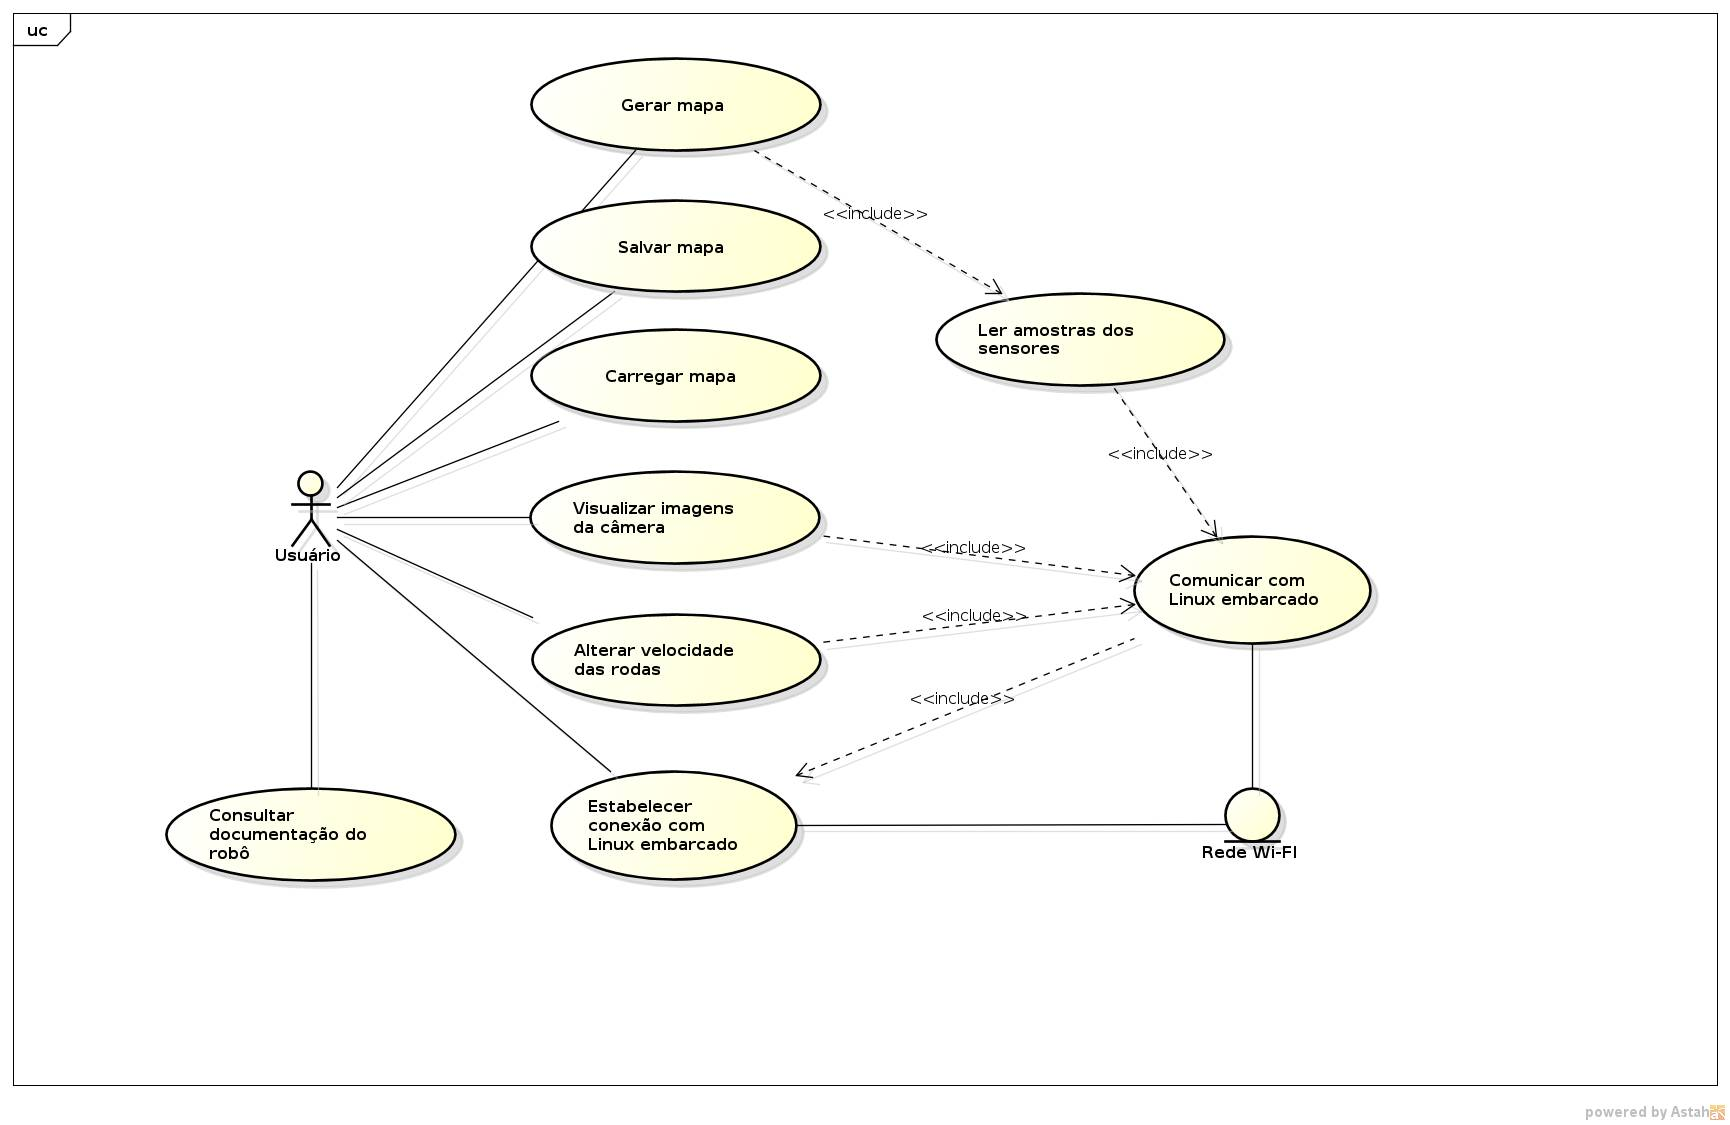
\includegraphics[width=\textwidth, keepaspectratio]{./figuras/estacaoBase/usecase_estacao_base.jpg}
  \caption{Diagrama de casos de uso do \textit{software} da estação base.}
  \label{fig:diagrama_caso_uso_estacao_base}
\end{figure}

\begin{figure}[H]
  \centering
  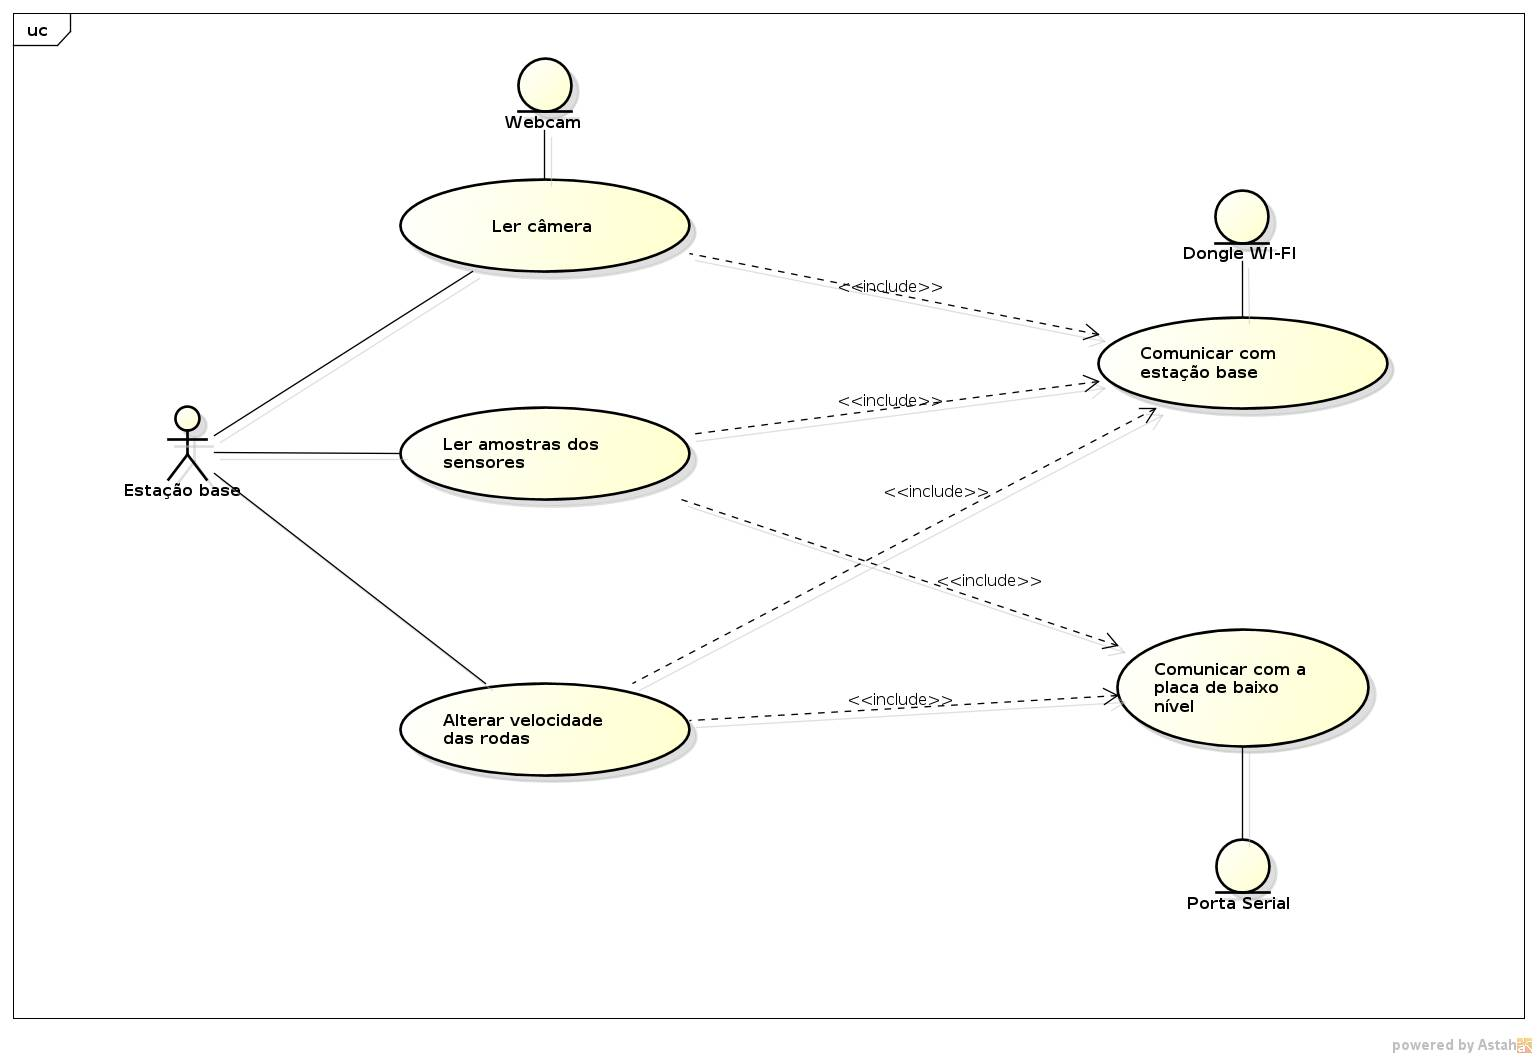
\includegraphics[width=\textwidth, keepaspectratio]{./figuras/sistEmbarcado/usecase_linux_embarcado.jpg}
  \caption{Diagrama de casos de uso do \textit{software} para a placa TS-7260.}
  \label{fig:diagrama_caso_uso_linux_embarcado}
\end{figure}

\begin{figure}[H]
  \centering
  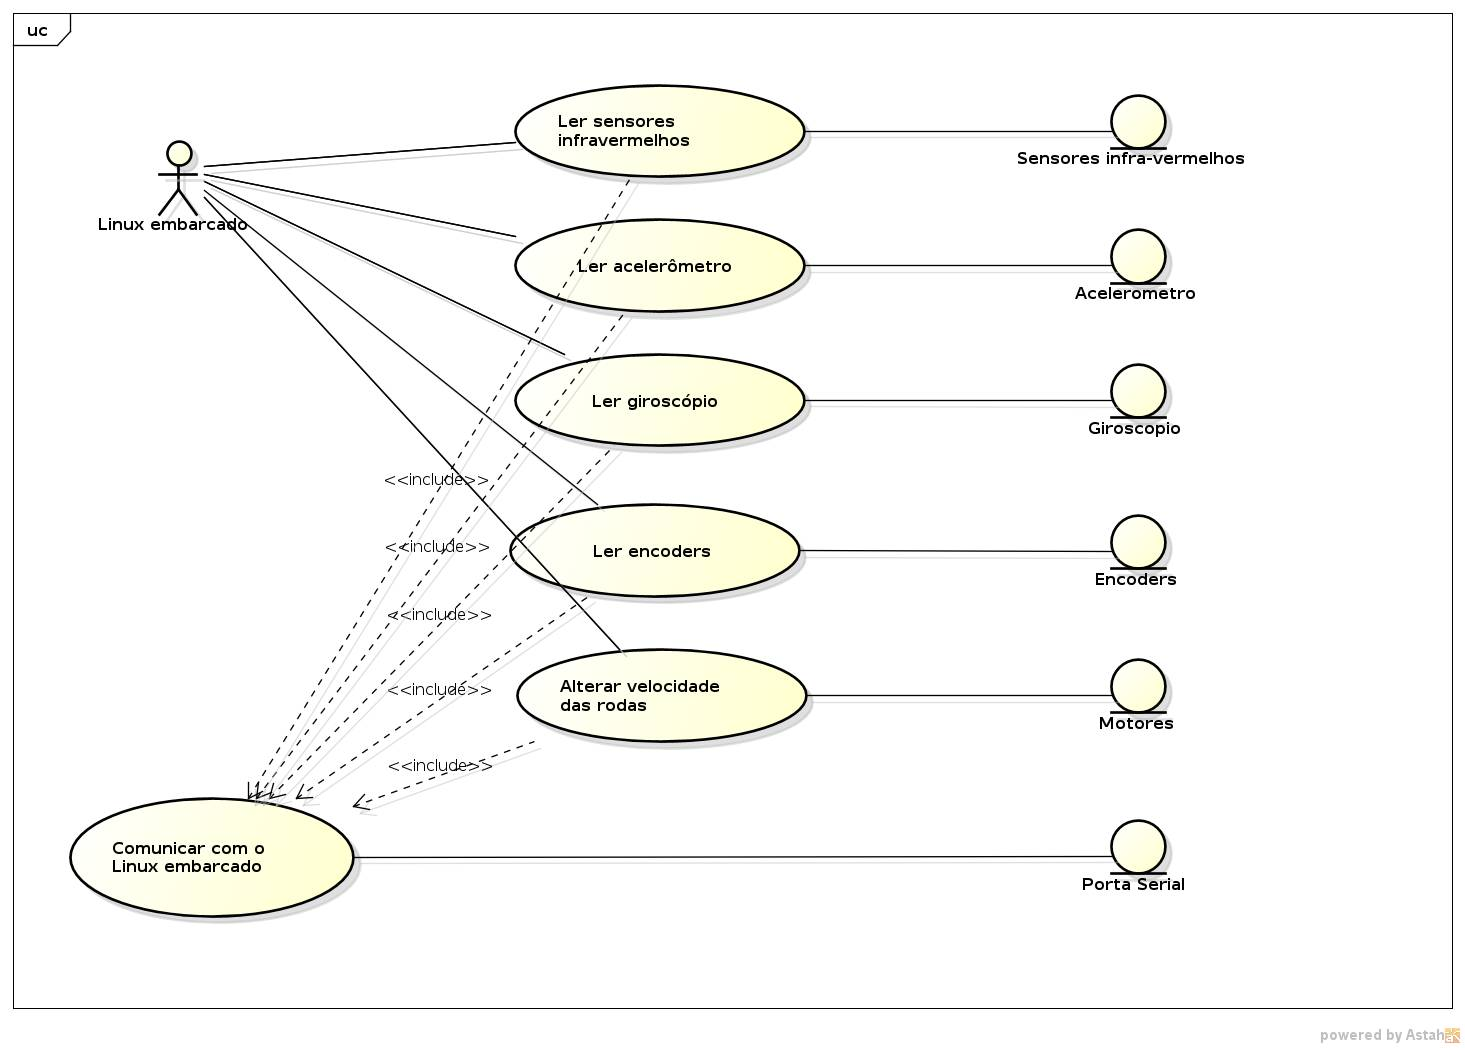
\includegraphics[width=\textwidth, keepaspectratio]{./figuras/sistEmbarcado/usecase_placa_baixo_nivel.jpg}
  \caption{Diagrama de casos de uso do \textit{software} para a placa de baixo nível.}
  \label{fig:diagrama_caso_uso_placa_embarcada}
\end{figure}

\subsection{Hardware}

Na figura \ref{fig:diagrama_blocos_hardware} mostra-se o diagrama de blocos do sistema embarcado e suas conexões com o restante do robô. A seguir está também uma descrição para cada um dos blocos da placa de circuito impresso do sistema embarcado.

\begin{figure}[H]
  \centering
  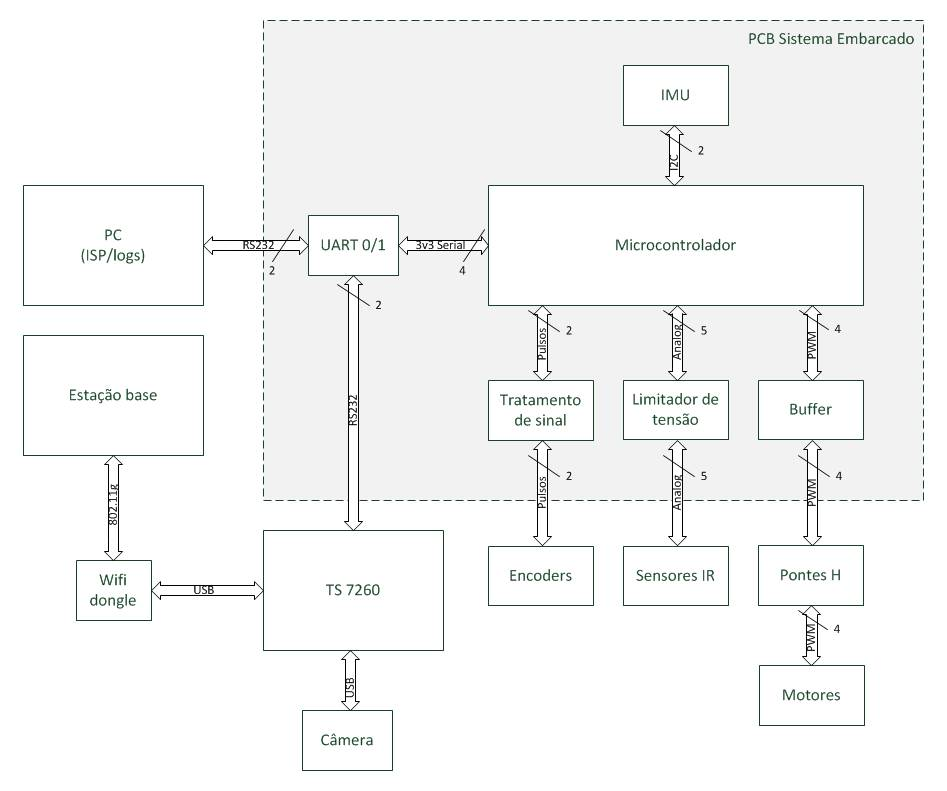
\includegraphics[width=\textwidth]{./figuras/hardware/diagrama_blocos_hardware.jpg}
  \caption{Diagrama de blocos do hardware}
  \label{fig:diagrama_blocos_hardware}
\end{figure}


\begin{enumerate}[topsep=0pt, partopsep=0pt, itemsep=0pt]
    \item Microcontrolador: Este bloco fará a leitura dos sensores: encoders, infra-vermelhos, acelerômetro e giroscópios. Além disso possui a implementação do protocolo de comunicação para interação com o linux embarcado da placa TS-7260.
    \item UART 0/1: Responsável por ajustar os níveis de tensão para comunicação serial no padrão RS-232 com a placa TS-7260.
    \item Buffer: Responsável por fornecer corrente e elevar os níveis de tensão de saída do microcontrolador de 3,3V para 5,0V. Esse buffer é conectado às pontes H já existentes no robô.
    \item IMU (Inertial Measurement Unit): possui o acelerômetro e o giroscópio e se comunicará com o microcontrolador por meio do protocolo I2C.
    \item Limitador de tensão: Necessário pois os sinais de saída dos sensores de infravermelho que já existem no robô não estão limitados em 5V, podendo a saída ultrapassar 5,0V e danificar o microcontrolador. 
    \item Tratamento de sinal: Composto por um filtro RC passa baixas e um Schmitt trigger para remover qualquer falha que possa ocorrer na geração dos pulsos no encoder.
\end{enumerate}

\section{Estação-base}
\subsection{Diagrama de classes da estação base}

A Figura \ref{fig:diagrama_classes_estacao_base} mostra o diagrama de classes da estação base.
\begin{figure}[H]
  \centering
  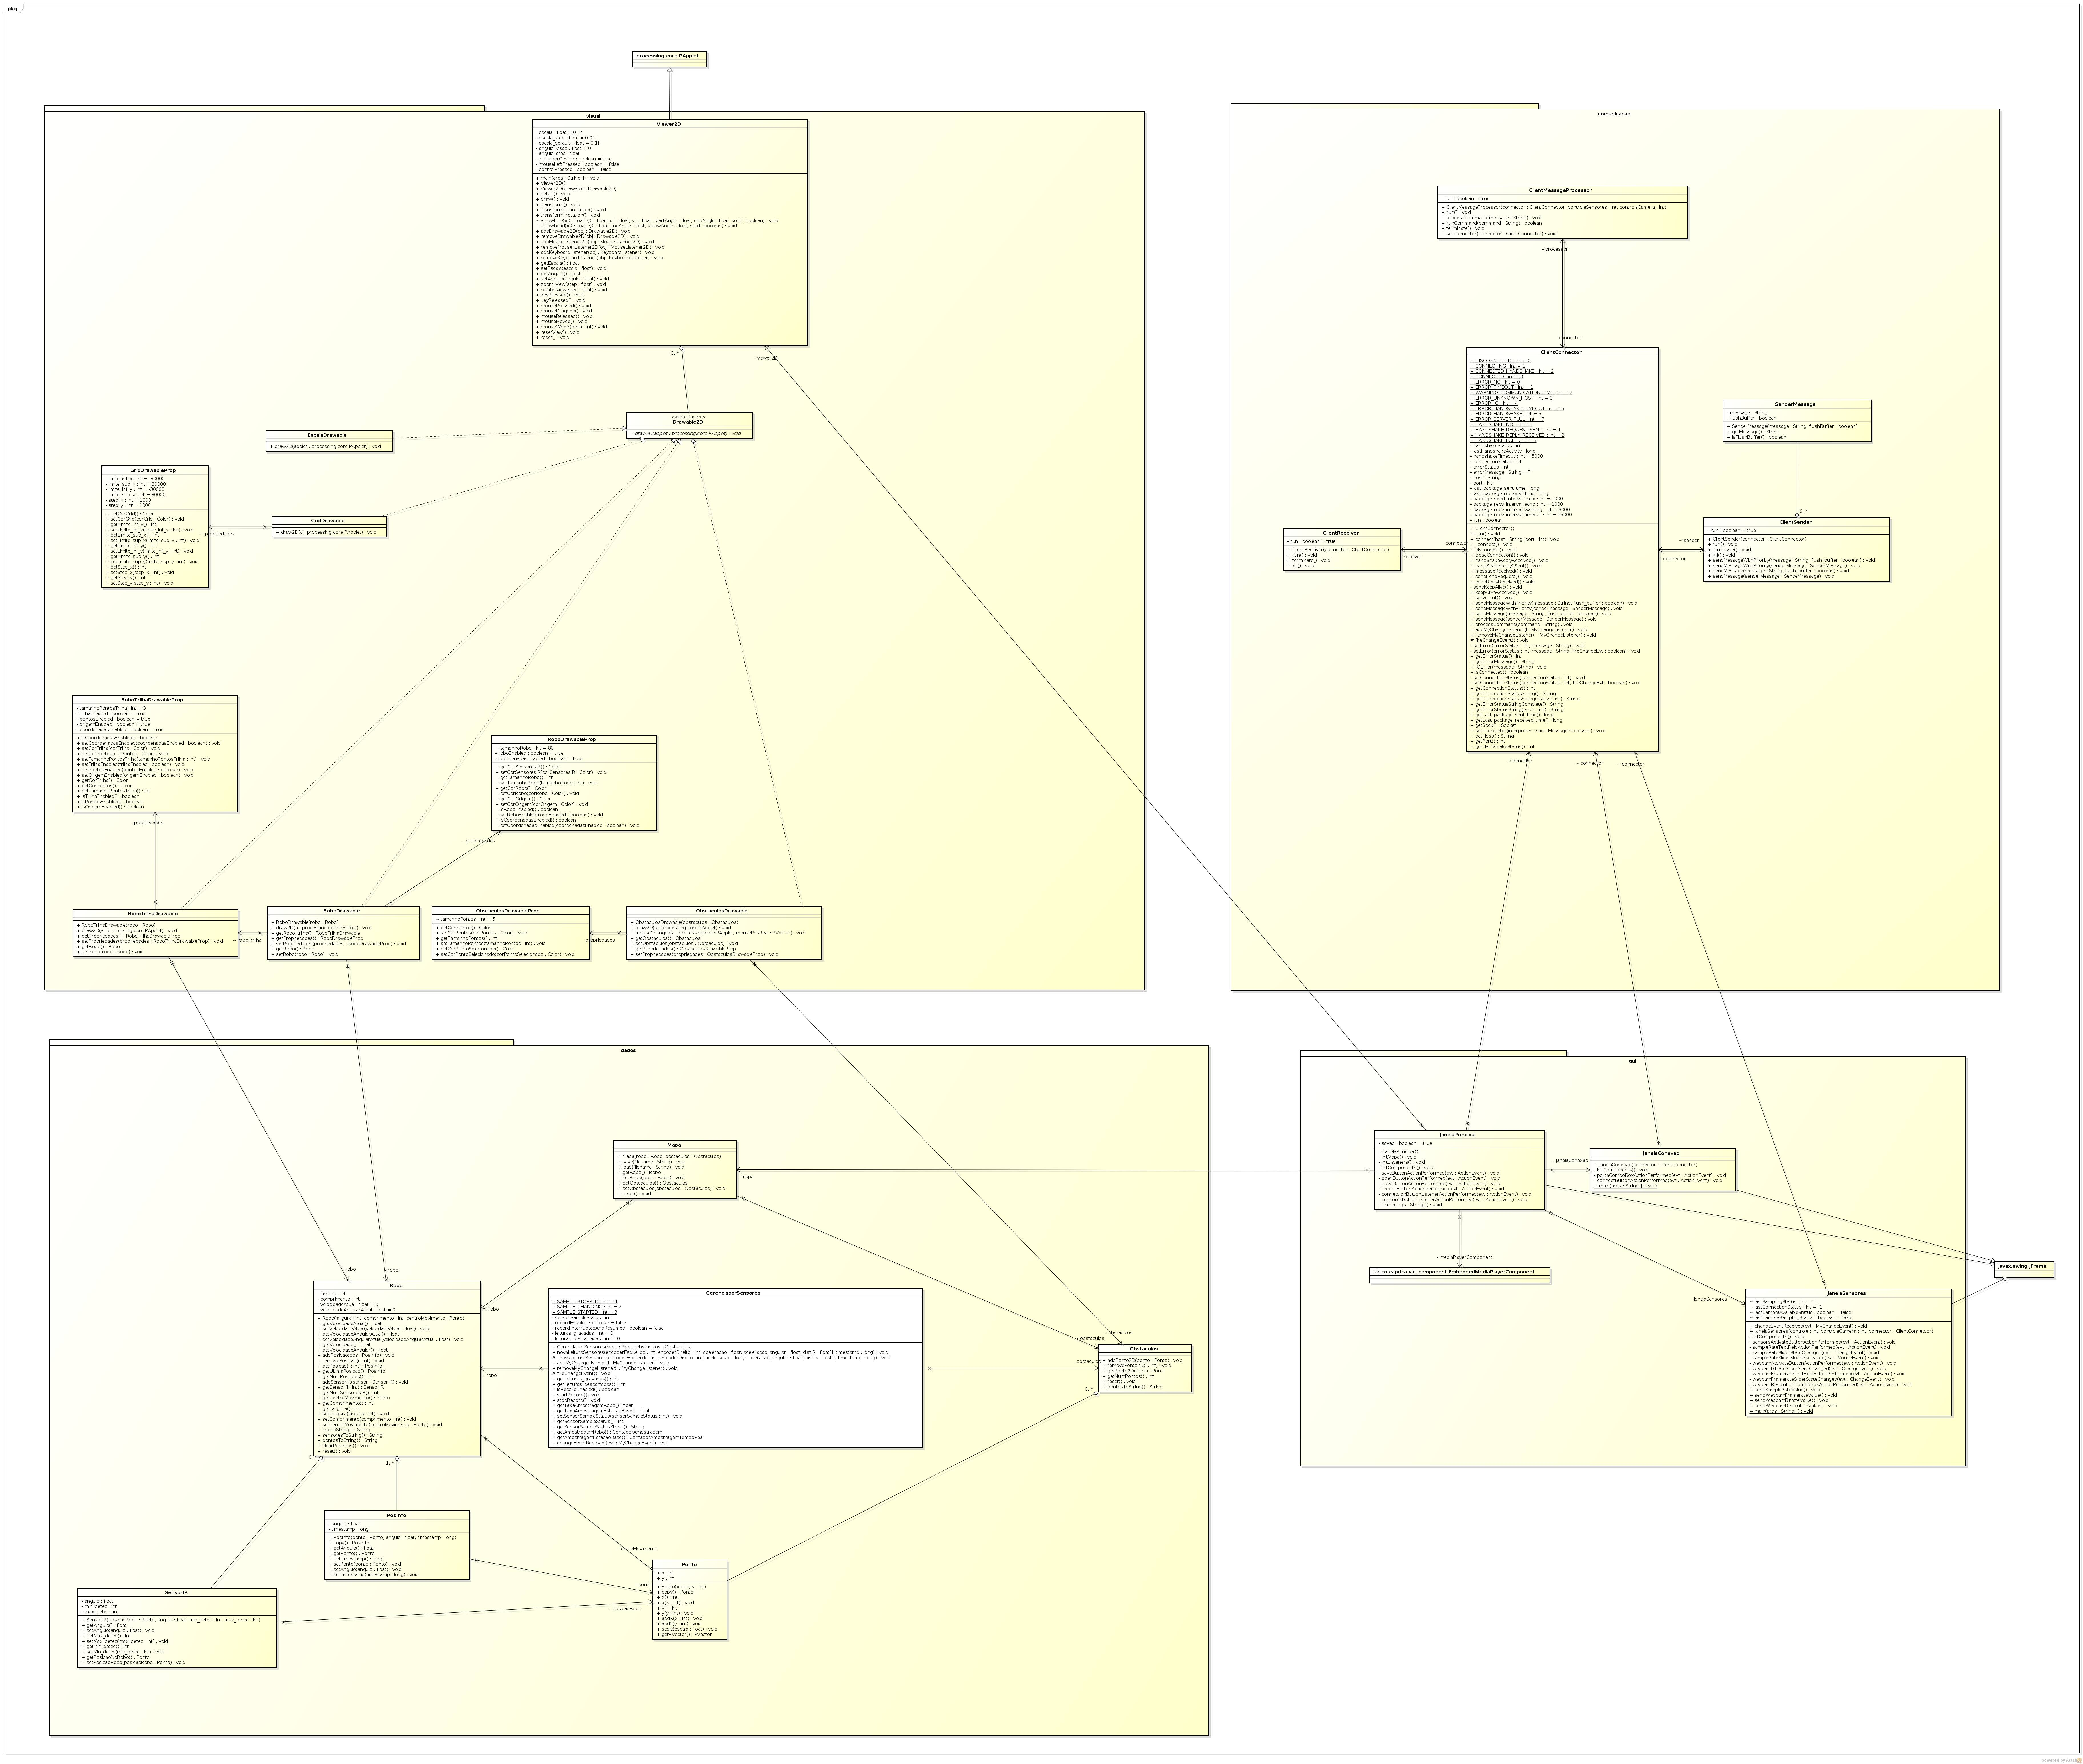
\includegraphics[width=\textwidth]{./figuras/estacaoBase/class_estacaoBase.jpg}
  \caption{Diagrama de classes da estação base}
  \label{fig:diagrama_classes_estacao_base}
\end{figure}

\subsubsection{Descrição das classes da estação base}
%O software da estação base do robô foi dividido em cinco pacotes:  visual, controle, comunicação, controle.robo e interface gráfica. Estes serão descritos com suas respectivas classes na Tabela \ref{tab:pacote_visual}.
O \textit{software} da estação base do robô foi dividido em cinco pacotes:  \textit{visual}, \textit{dados}, \textit{comunicacao}, e \textit{gui}. A seguir há uma descrição de cada pacote e das suas respectivas classes.


\subsubsection{Pacote \textit{visual}}

Este pacote consiste de toda a parte visual da estação base e conta com as seguintes classes: Viewer2D, Drawable2D, EscalaDrawable, RoboDrawable, RoboTrilhaDrawable, ObstaculosDrawable, EscalaDrawableProp, RoboDrawableProp, RoboTrilhaDrawableProp e ObstaculosDrawableProp. Na Tabela \ref{tab:pacote_visual} estão descritas as classes deste pacote.


\begin{table}[H]
  \centering
  \caption{Pacote \textit{visual}}
  \begin{tabular}{p{6cm}p{8cm}}
    \toprule
    \textbf{Classe} & \textbf{Descrição} \\
    \midrule
    Viewer2D & Responsável por exibir os objetos Drawable2D. Possui recursos de pan, zoom e rotate.   \\ \hline
    Drawable2D & Representa genericamente objetos 2D que podem ser desenhados em um Viewer2D. \\ \hline
    EscalaDrawable & Responsável por desenhar uma escala gráfica no mapa. \\ \hline
    RoboDrawable & Responsável por desenhar o robô no mapa. \\ \hline
    RoboTrilhaDrawable & Responsável por desenhar a trilha percorrida pelo robô no mapa. \\ \hline
    ObstaculosDrawable & Responsável por desenhar os pontos de cada obstáculo no mapa. \\ \hline
    EscalaDrawableProp & Contém as propriedades visuais de desenho da escala. \\ \hline
    RoboDrawableProp & Contém as propriedades visuais de desenho do robô \\ \hline
    RoboTrilhaDrawableProp & Contém as propriedades visuais de desenho da trilha do robô. \\ \hline
    ObstaculosDrawableProp & Contém as propriedades visuais de desenho dos obstáculos. \\
    \bottomrule
  \end{tabular}%
  \label{tab:pacote_visual}%
\end{table}%

\subsubsection{Pacote \textit{dados}}

Este pacote consiste de toda a parte da estação base que processa e armazena as informações essenciais do robô e do mapa. Conta com as seguintes classes: Mapa, Obstaculos, Robo, ControleSensores, Posinfo, SensorIR e Ponto. Na Tabela \ref{tab:pacote_controle} estão descritas as classes deste pacote.

\begin{table}[H]
  \centering
  \caption{Pacote \textit{dados}}
  \begin{tabular}{p{6cm}p{8cm}}
    \toprule
    \textbf{Classe} & \textbf{Descrição} \\ 
    \midrule
    Mapa  & Responsável por representar o mapa. Armazena as informações essenciais do robô e dos obstáculos detectados. \\ \hline
    Obstaculos & Responsável por conter os obstáculos detectados pelo robô. \\ \hline
    Robo  & Responsável por representar o robô, este contêm largura, comprimento e centro de movimento (ponto central entre as duas rodas). \\ \hline
    GerenciadorSensores & Responsável por atualizar a posição do robô e dos pontos que representam os obstáculos, de acordo com as leituras feitas pelos sensores. \\ \hline
    Posinfo & Responsável por conter as informações de uma posição do robô. \\ \hline
    SensorIR & Responsável por representar um sensor IR do robô. \\ \hline 
    Ponto & Representa um ponto de cordenadas cartesianas (x,y). \\ \hline
    GerenciadorCamera & Responsável por gerenciar o status da câmera e o recebimento de imagens. \\ 
    \bottomrule
  \end{tabular}%
  \label{tab:pacote_controle}%
\end{table}%

\subsubsection{Pacote \textit{comunicacao}}
\label{subsec:pacote_comunicacao}

%Este pacote consiste em toda a parte de comunicação da estação base com o robô e conta com as seguintes classes: ClientCommandInterpreter, ClientConnection, ClientReceiver, ClientSender, ServerCommandInterpreter, ServerListener, ServerSender, ServerReceiver e Message. Na Tabela \ref{tab:pacote_comunicacao} estão descritas as classe deste pacote.
Este pacote consiste em toda a parte de comunicação da estação base com o robô e conta com as seguintes classes: ClientMessageProcessor ClientConnection, ClientReceiver, ClientSender e Message. Na Tabela \ref{tab:pacote_comunicacao} estão descritas as classes deste pacote.

É importante ressaltar que o protocolo TCP requer obrigatoriamente a especificação de um cliente e de um servidor para estabelecimento de uma conexão. Nas implementações desse protocolo em diversas linguagens (como Java e C++) existem tipos de \textit{socket} distintos para cliente e servidor. Na criação de um \textit{socket} de servidor, há obrigatoriamente a atribuição de uma porta de escuta, na qual o servidor aguarda que um cliente efetue uma requisição de conexão. Não é possível, ao menos nas implementações atuais do TCP, estabelecer conexão entre dois \textit{sockets} de cliente ou entre dois \textit{sockets} de servidor. Como neste projeto, o robô proverá serviços à estação base (envio de imagens da câmera, envio de leituras de sensores, além de prover a possibilidade de comando dos motores) o robô foi escolhido como servidor e a estação base como cliente. Enfatiza-se que o paradigma cliente-servidor não implica de forma alguma que a comunicação seja unidirecional. Pelo contrário, o envio de pacotes 
pode ser feito bidirecionalmente após uma conexão TCP ser estabelecida, sem nenhuma restrição quanto a isso.

\begin{table}[H]
  \centering
  \caption{Pacote \textit{comunicacao}}
  \begin{tabular}{p{6cm}p{8cm}}
    \toprule
    \textbf{Classe} & \textbf{Descrição} \\ 
    \midrule
    ClientMessageProcessor & Thread responsável pelo processamento de mensagens recebidas de um host de conexão. \\ \hline
    ClientConnector & Thread responsável por efetuar a gerência da conexão do cliente (estação base) com o servidor (robô). \\ \hline
    ClientReceiver & Thread responsável por receber mensagens de um host de uma conexão. \\ \hline
    ClientSender & Thread responsável por enviar mensagens ao host de uma conexão. \\ \hline
%    ServerCommandInterpreter & Responsável pela interpretação dos comandos do servidor. Os comandos recebidos são inseridos em uma fila, de modo a serem posteriormente executados pela thread. \\ \hline
%    Server & Responsável gerenciar o servidor (robô). \\ \hline
%    ServerListener & Responsável por escutar as novas conexões de clientes. \\ \hline
%    ServerSender & Responsável por enviar mensagens ao host de uma conexão. \\ \hline
%    ServerReceiver & Responsável por receber mensagens de um host de uma conexão. \\ \hline
    SenderMessage & Contém uma mensagem que pode ser enviada por um Sender. \\ \hline
    \bottomrule
  \end{tabular}%
  \label{tab:pacote_comunicacao}%
\end{table}%

\subsubsection{Pacote \textit{gui}}

Este pacote consiste em toda a interface gráfica do sistema e conta com as seguintes classes: JanelaConexao, JanelaPrincipal e JanelaSensores. Na Tabela \ref{tab:pacote_interface_grafica} estão descritas as classes deste pacote.

\begin{table}[H]
  \centering
  \caption{Pacote \textit{gui}}
  \begin{tabular}{p{6cm}p{8cm}}
    \toprule
    \textbf{Classe} & \textbf{Descrição} \\ 
    \midrule
    JanelaConexao & Janela com as informações e configurações da conexão com o Bellator. \\ \hline
    JanelaPrincipal & Janela principal da interface gráfica da estação base. \\ \hline
    JanelaSensores & Janela de configuração dos sensores. \\ 
    \bottomrule
  \end{tabular}%
  \label{tab:pacote_interface_grafica}%
\end{table}%

% \section{Fluxo de dados}
% 
% A Figura \ref{fig:diagrama_fluxo_dados} mostra o diagrama de fluxo de dados.
% 
% \begin{figure}[H]
%   \centering
%   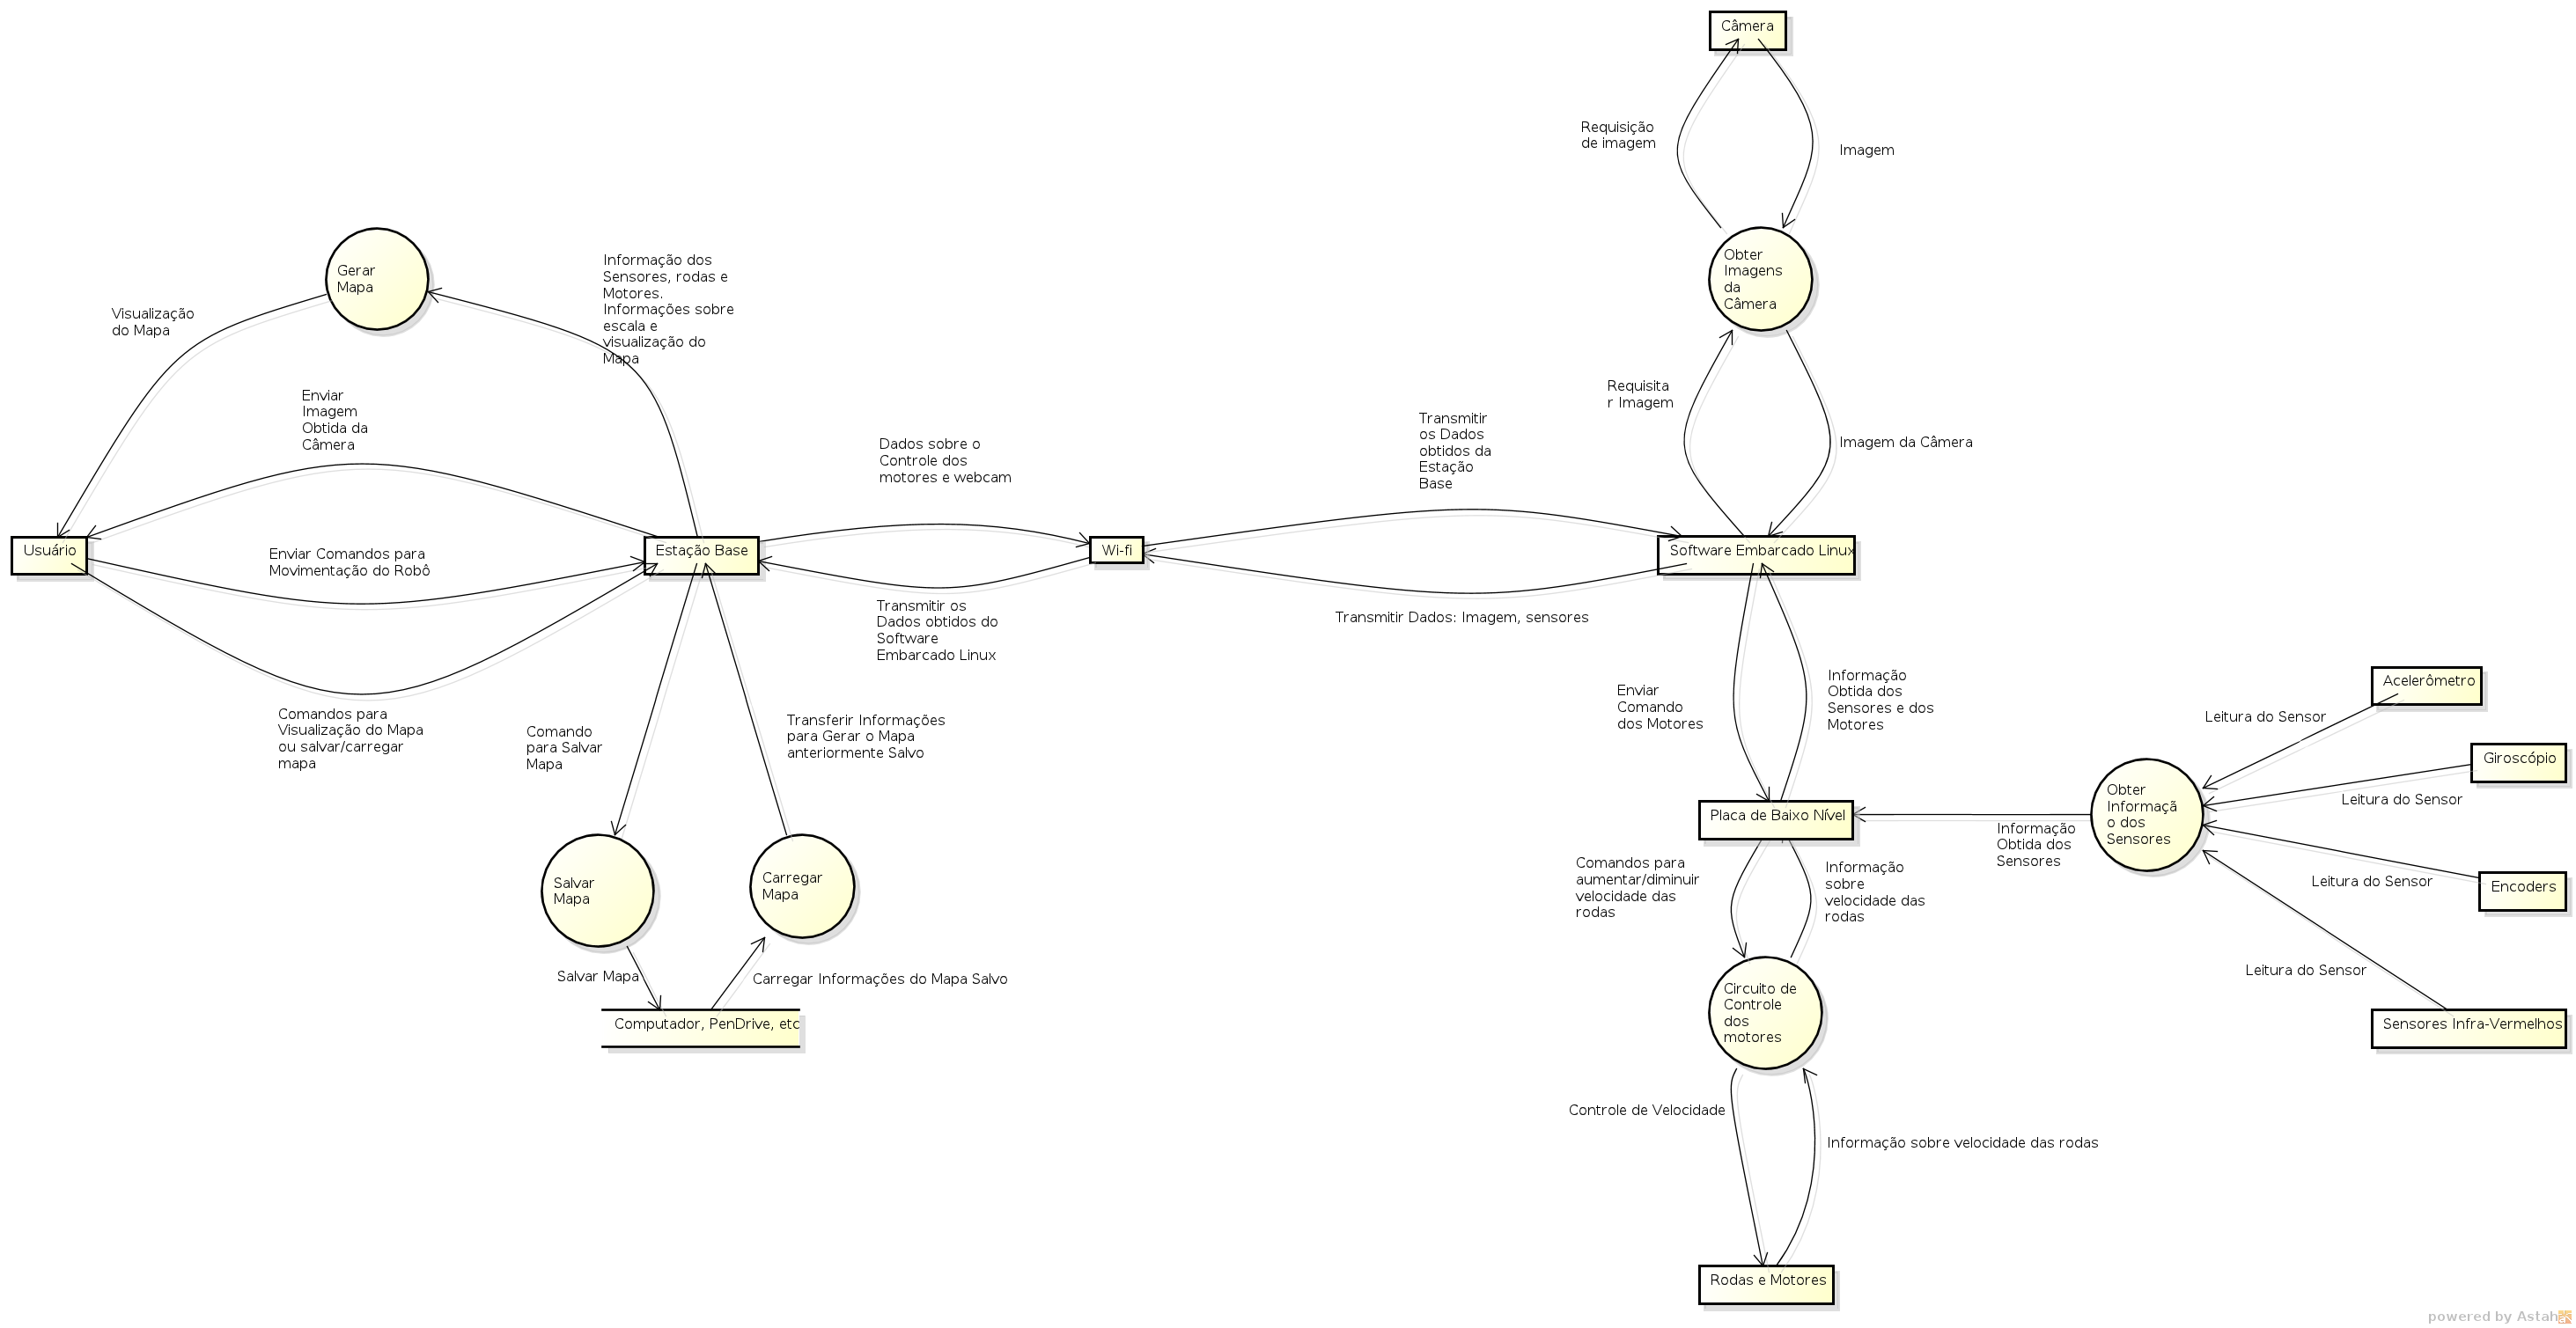
\includegraphics[width=\textwidth, keepaspectratio]{./figuras/diagrama_fluxo_dados.jpg}
%   \caption{Diagrama de fluxo de dados.}
%   \label{fig:diagrama_fluxo_dados}
% \end{figure}

% \section{Diagrama de estados}
% As Figuras \ref{fig:diagrama_estados_estacao_base} e \label{fig:diagrama_estados_sistema_embarcado} mostram os diagramas de estados do sistema.
% 
% \begin{figure}[H]
%   \centering
%   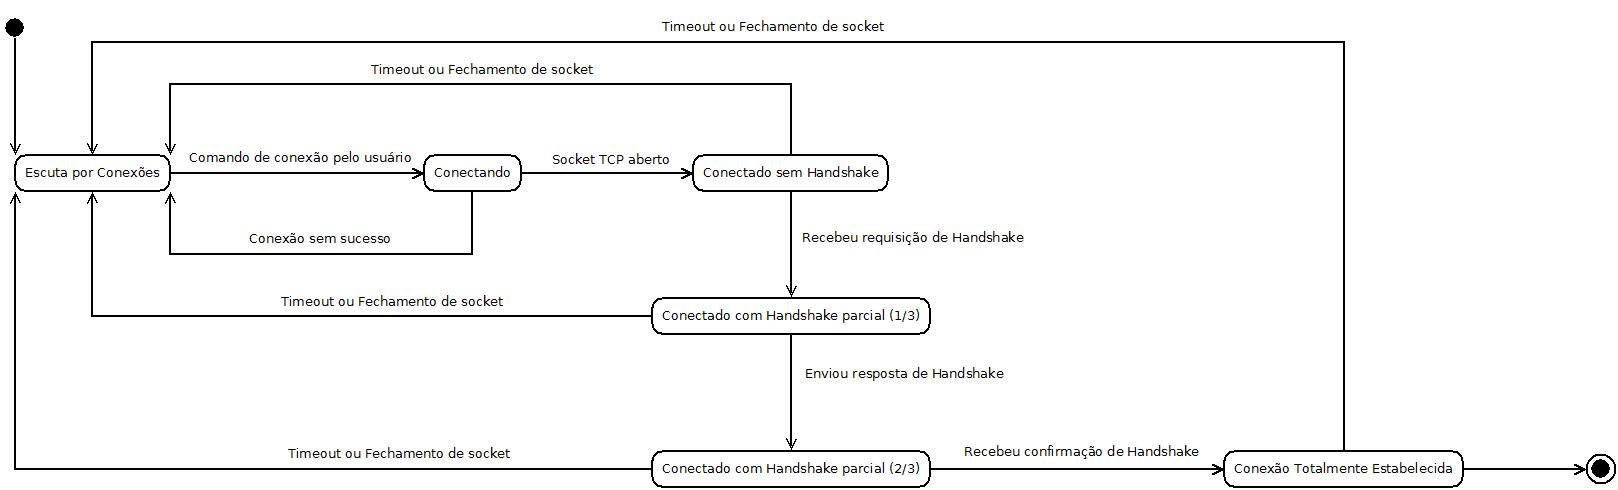
\includegraphics[width=\textwidth, keepaspectratio]{./figuras/diagrama_estados_estacao_base.jpeg}
%   \caption{Diagrama de estados para a estação base.}
%   \label{fig:diagrama_estados_estacao_base}
% \end{figure}
% 
% \begin{figure}[H]
%   \centering
%   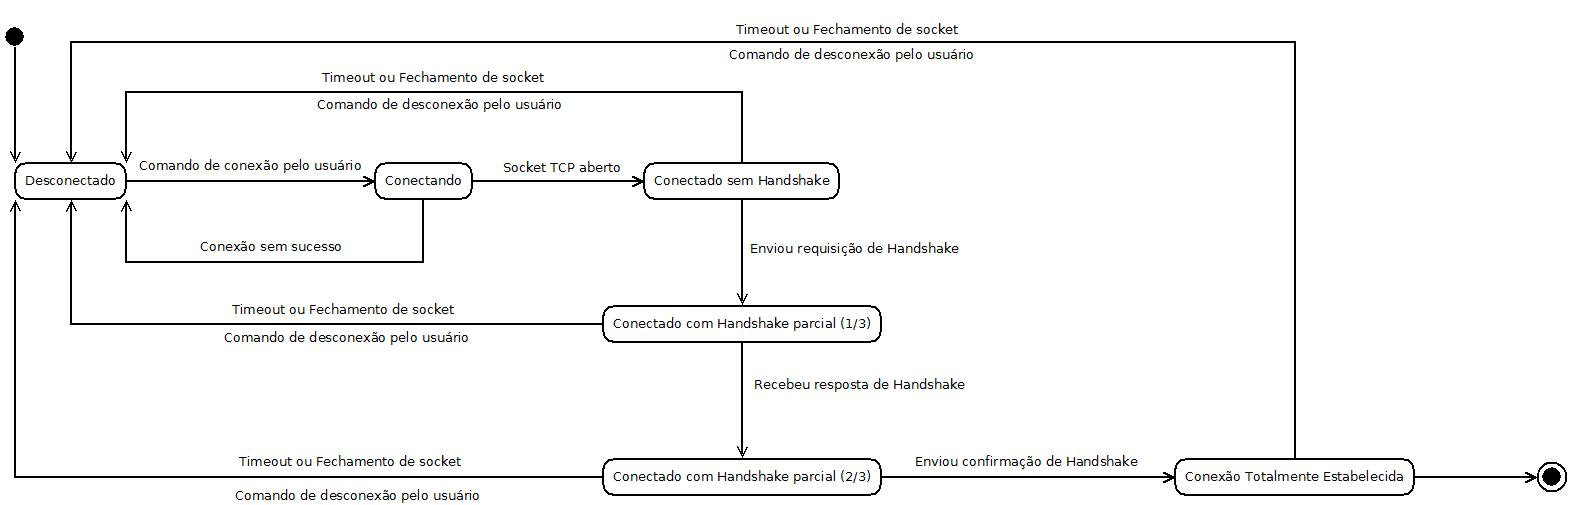
\includegraphics[width=\textwidth, keepaspectratio]{./figuras/diagrama_estados_sistema_embarcado.jpeg}
%   \caption{Diagrama de estados para o sistema embarcado.}
%   \label{fig:diagrama_estados_sistema_embarcado}
% \end{figure}

\section{Sistema de comunicação}
\subsection{Codificação das mensagens}
\label{sec:codificacao_mensagens}

\begin{itemize}
  \item Mensagens do TS-7260 para o LPC2103 (via porta serial)
    	
	\begin{itemize}
		
	  \item \textbf{SYNC (0xA0)}\\
	  Quando o microcontrolador LPC2103 recebe esta mensagem, responde com as leituras mais recentes dos encoders, de cada sensor de distância, do acelerômetro e do giroscópio (enviando uma mensagem SENSORS, explicada abaixo).
	  
	  \item \textbf{ENGINES (0xB0)}\\
	  \textit{(byte) vel\_roda\_esquerda}\\
	  \textit{(byte) vel\_roda\_direita}\\
	  \textit{(byte) CHECKSUM\_H}\\
	  \textit{(byte) CHECKSUM\_L}\\
	  Ao receber este comando, o microcontrolador utiliza os valores para definir o nível de PWM para as rodas do robô. Os valores de velocidade são representados por um byte cada, nos quais o bit mais significativo indica o sentido de rotação da roda (1 para frente e 0 para trás) e os restantes a intensidade do PWM.
	  
	  Os bytes de checksum são utilizados para verificar se não há dados corrompidos. Os bytes da mensagem são somados (módulo 65536) e o resultado é atribuído aos bytes (high e low) de checksum.
	  \end{itemize}
	  
	  \item Mensagens do LPC2103 para a TS-7260 (via porta serial)
	  
	  \begin{itemize}

	  \item \textbf{ENGINES\_ACK (0xB1)}\\
	  \textit{(byte) vel\_roda\_esquerda}\\
	  \textit{(byte) vel\_roda\_direita}\\
	  \textit{(byte) CHECKSUM\_H}\\
	  \textit{(byte) CHECKSUM\_L}\\
	  Esta mensagem deve ser enviada toda vez que um comando de mudança de velocidade (ENGINES) for recebido na placa de baixo nível. A mensagem é usada no Linux embarcado para verificar se o comando foi corretamente recebido. Caso uma confirmação não seja recebida em certo intervalo de tempo, outro comando ENGINES é enviado para a placa de baixo nível.
	 
	  O checksum tem função idêntica ao que já foi explicitado na mensagem ENGINES.
	  
	  \item \textbf{SENSORS (0xC0)}\\
	  \textit{(byte) encoder\_esq\_H}, \textit{(byte) encoder\_esq\_L},\\
	  \textit{(byte) encoder\_dir\_H}, \textit{(byte) encoder\_dir\_L},\\
	  \textit{(byte) IR1}, \textit{(byte) IR2}, \textit{(byte) IR3}, \textit{(byte) IR4}, \textit{(byte) IR5},\\
	  \textit{(byte) AX\_H}, \textit{(byte) AX\_L},\\
	  \textit{(byte) AY\_H}, \textit{(byte) AY\_L},\\
	  \textit{(byte) AZ\_H}, \textit{(byte) AZ\_L},\\
	  \textit{(byte) GX\_H}, \textit{(byte) GX\_L},\\
	  \textit{(byte) GY\_H}, \textit{(byte) GY\_L},\\
	  \textit{(byte) GZ\_H}, \textit{(byte) GZ\_L},\\
	  \textit{(byte) TIMESTAMP\_H}, \textit{(byte) TIMESTAMP\_L}\\
	  \textit{(byte) CHECKSUM\_H}\\
	  \textit{(byte) CHECKSUM\_L}\\
	  Representa a leitura de todos os sensores (encoders, infra-vermelhos, acelerômetro e giroscópio). 
	  
	  Os 4 primeiros bytes são os valores das leituras dos encoders esquerdo e direito (cada um com um byte alto e um baixo). Os valores das leituras dos encoders representam a diferença entre a contagem atual a contagem anterior.
	  
	  Nos próximos 5 bytes, as leituras do sensores ópticos são enviadas em sequência. As distâncias que os sensores ópticos são capazes de mensurar são divididos em valores discretos de 0 a 255 \cite{bellator_2012}. 
	  
	  Após isso, os 12 bytes que se seguem representam as leituras do acelerômetro e do giroscópio. Os bytes que começam com `A' representam a leitura de cada um dos eixos do acelerômetro. Aqueles que começam com `G' representam a leitura de cada um dos eixos do giroscópio.
	  
	  O timestamp (valor alto e baixo) é um contador de 16 bits que é incrementado entre cada amostra e zera automaticamente depois que chega ao valor máximo (65535), usado para determinar o instante em que foi feita a leitura dos dados. Como a amostragem dos sensores na placa de baixo nível será efetuada em intervalos fixos, a informação do contador do timestamp pode ser utilizada para obter informações de tempo de cada amostra.

	  O checksum é tem função idêntica ao que já foi explicitado na mensagem ENGINES.
	  
	  
	\end{itemize}

  \item Mensagens bidirecionais entre estação base e TS-7260 (via WI-Fi):

    \begin{itemize}
      \item \textbf{ECHO\_REQUEST (0x01)}\\
      \textit{(byte) END\_CMD}\\
	Requisição de ping.
      \item \textbf{ECHO\_REPLY (0x02)}\\
      \textit{(byte) END\_CMD}\\
	Resposta de ping.
      \item \textbf{DISCONNECT (0x0F)} \\
	Solicitação de desconexão.
    \end{itemize}

  \item Mensagens da estação base para a TS-7260 (via Wi-Fi):

    \begin{itemize}
      \item \textbf{HANDSHAKE\_REQUEST (0x10)}\\
	Solicitação de handshake.

      \item \textbf{HANDSHAKE\_CONFIRMATION (0x12)}\\
	Confirmação de handshake.

      \item \textbf{SENSORS\_START (0x20)}\\
	Solicitação de início da amostragem dos sensores.

      \item \textbf{SENSORS\_STOP (0x21)}\\
	Solicitação de parada da amostragem dos sensores.

      \item \textbf{SENSORS\_RATE (0x22)} \\
	\textit{(float) Nova taxa de amostragem (comandos SYNC por segundo)}\\
	Solicitação de mudança da taxa de envio de comandos SYNC da TS para a placa de baixo nível.

%       \item \textbf{SENSORS\_STATUS\_REQUEST}\\
%       \textit{(byte) END\_CMD}\\
% 	Requisição de status da amostragem dos sensores. Usado na interface gráfica para atualizar as informações sobre os sensores.

      \item \textbf{WEBCAM\_START (0x30)}\\
	Solicitação de início da amostragem da webcam.

      \item \textbf{WEBCAM\_STOP (0x31)}\\
	Solicitação de parada da amostragem da webcam.

      \item \textbf{WEBCAM\_RATE (0x32)} \\
	\textit{(float) Nova taxa de quadros}\\
	Solicitação de mudança da taxa de quadros da webcam.

      \item \textbf{WEBCAM\_RESOLUTION (0x33)} \\
	\textit{(int) Largura em pixels }\\
	\textit{(int) Altura em pixels}\\
	Solicitação de mudança da resolução da webcam.

%       \item \textbf{WEBCAM\_STATUS\_REQUEST}\\
%       \textit{(byte) END\_CMD}\\
% 	Solicitação de informações sobre status da webcam. Usado na interface gráfica para atualizar as informações sobre a webcam.

      \item \textbf{ENGINES (0xB0)} \\
	 \textit{(float) vel\_roda\_esquerda}\\
	 \textit{(float) vel\_roda\_direita}\\
	Solicitação de mudança da velocidade dos motores. Para cada roda há um valor de -1 até 1, sendo que -1 é a máxima velocidade para trás, 1 a máxima velocidade para frente e 0 é parada da roda.

%       \item \textbf{ENGINES\_STATUS\_REQUEST}\\
%       \textit{(byte) END\_CMD}\\
% 	Solicitação de status dos motores. Usado na interface gráfica para confirmar o recebimento de comandos de movimentação efetuados pelo usuário.

    \end{itemize}

  \item Mensagens da TS-7260 para a estação base (via Wi-Fi):

    \begin{itemize}
      \item \textbf{HANDSHAKE\_REPLY (0x11)}\\
	Resposta de handshake.
	
	 \item \textbf{SENSORS (0xC0)}\\
	  \textit{(byte) encoder1\_H}, \textit{(byte) encoder1\_L},\\
	  \textit{(byte) encoder2\_H}, \textit{(byte) encoder2\_L},\\
	  \textit{(byte) IR1}, \textit{(byte) IR2}, \textit{(byte) IR3}, \textit{(byte) IR4}, \textit{(byte) IR5},\\
	  \textit{(byte) AX\_H}, \textit{(byte) AX\_L},\\
	  \textit{(byte) AY\_H}, \textit{(byte) AY\_L},\\
	  \textit{(byte) AZ\_H}, \textit{(byte) AZ\_L},\\
	  \textit{(byte) GX\_H}, \textit{(byte) GX\_L},\\
	  \textit{(byte) GY\_H}, \textit{(byte) GY\_L},\\
	  \textit{(byte) GZ\_H}, \textit{(byte) GZ\_L},\\
	  \textit{(byte) TIMESTAMP\_H}, \textit{(byte) TIMESTAMP\_L}\\
	  
	  Possui a mesma funcionalidade e parâmetros que a mensagem SENSORS enviada da LPC2103 para a TS-7260, com exceção do timestamp, que é trocado por um timestamp UNIX em milissegundos (que representa o horário absoluto em que a amostra foi obtida na placa de baixo nível). Essa informação de tempo é utilizada pela estação base para efetuar os cálculos de posicionamento do robô.

      \item \textbf{SENSORS\_STATUS (0xC1)} \\
	\textit{(boolean) Status da amostragem [on - off] }\\
	\textit{(float) Taxa de amostragem}\\
	Informações de status dos sensores. Usado na interface gráfica para confirmar o recebimento de comandos de mudança de taxa de amostragem e início/parada da amostragem.

      \item \textbf{WEBCAM\_STATUS (0x34)} \\
% 	\textit{(boolean) Nova taxa de amostragem }\\
	\textit{(float) Taxa de quadros }\\
	\textit{(int) Largura em pixels }\\
	\textit{(int) Altura em pixels }\\
	\textit{(boolean) Status da stream [on - off] }\\
	\textit{(int) Porta da stream}\\
	Informações de status da webcam. Usado na interface gráfica para confirmar o recebimento de comandos relativos à webcam, e para que a estação base tenha conhecimento do status da stream da webcam.
	
      \item \textbf{ENGINES\_STATUS (0xB1)} \\
	\textit{(byte) vel\_roda\_esquerda}\\
	\textit{(byte) vel\_roda\_direita}\\
	Informações sobre as velocidades programadas dos motores. Usado na interface gráfica para confirmar o recebimento de comandos de movimentação efetuados pelo usuário.

	

    \end{itemize}
\end{itemize}


\section{Sistema embarcado}
\subsection{Diagram de classes do sistema embarcado}
A Figura \ref{fig:diagrama_classes_sist_embarcado} mostra o diagrama de classes do sistema embarcado (placa TS-7260).
\begin{figure}[H]
  \centering
  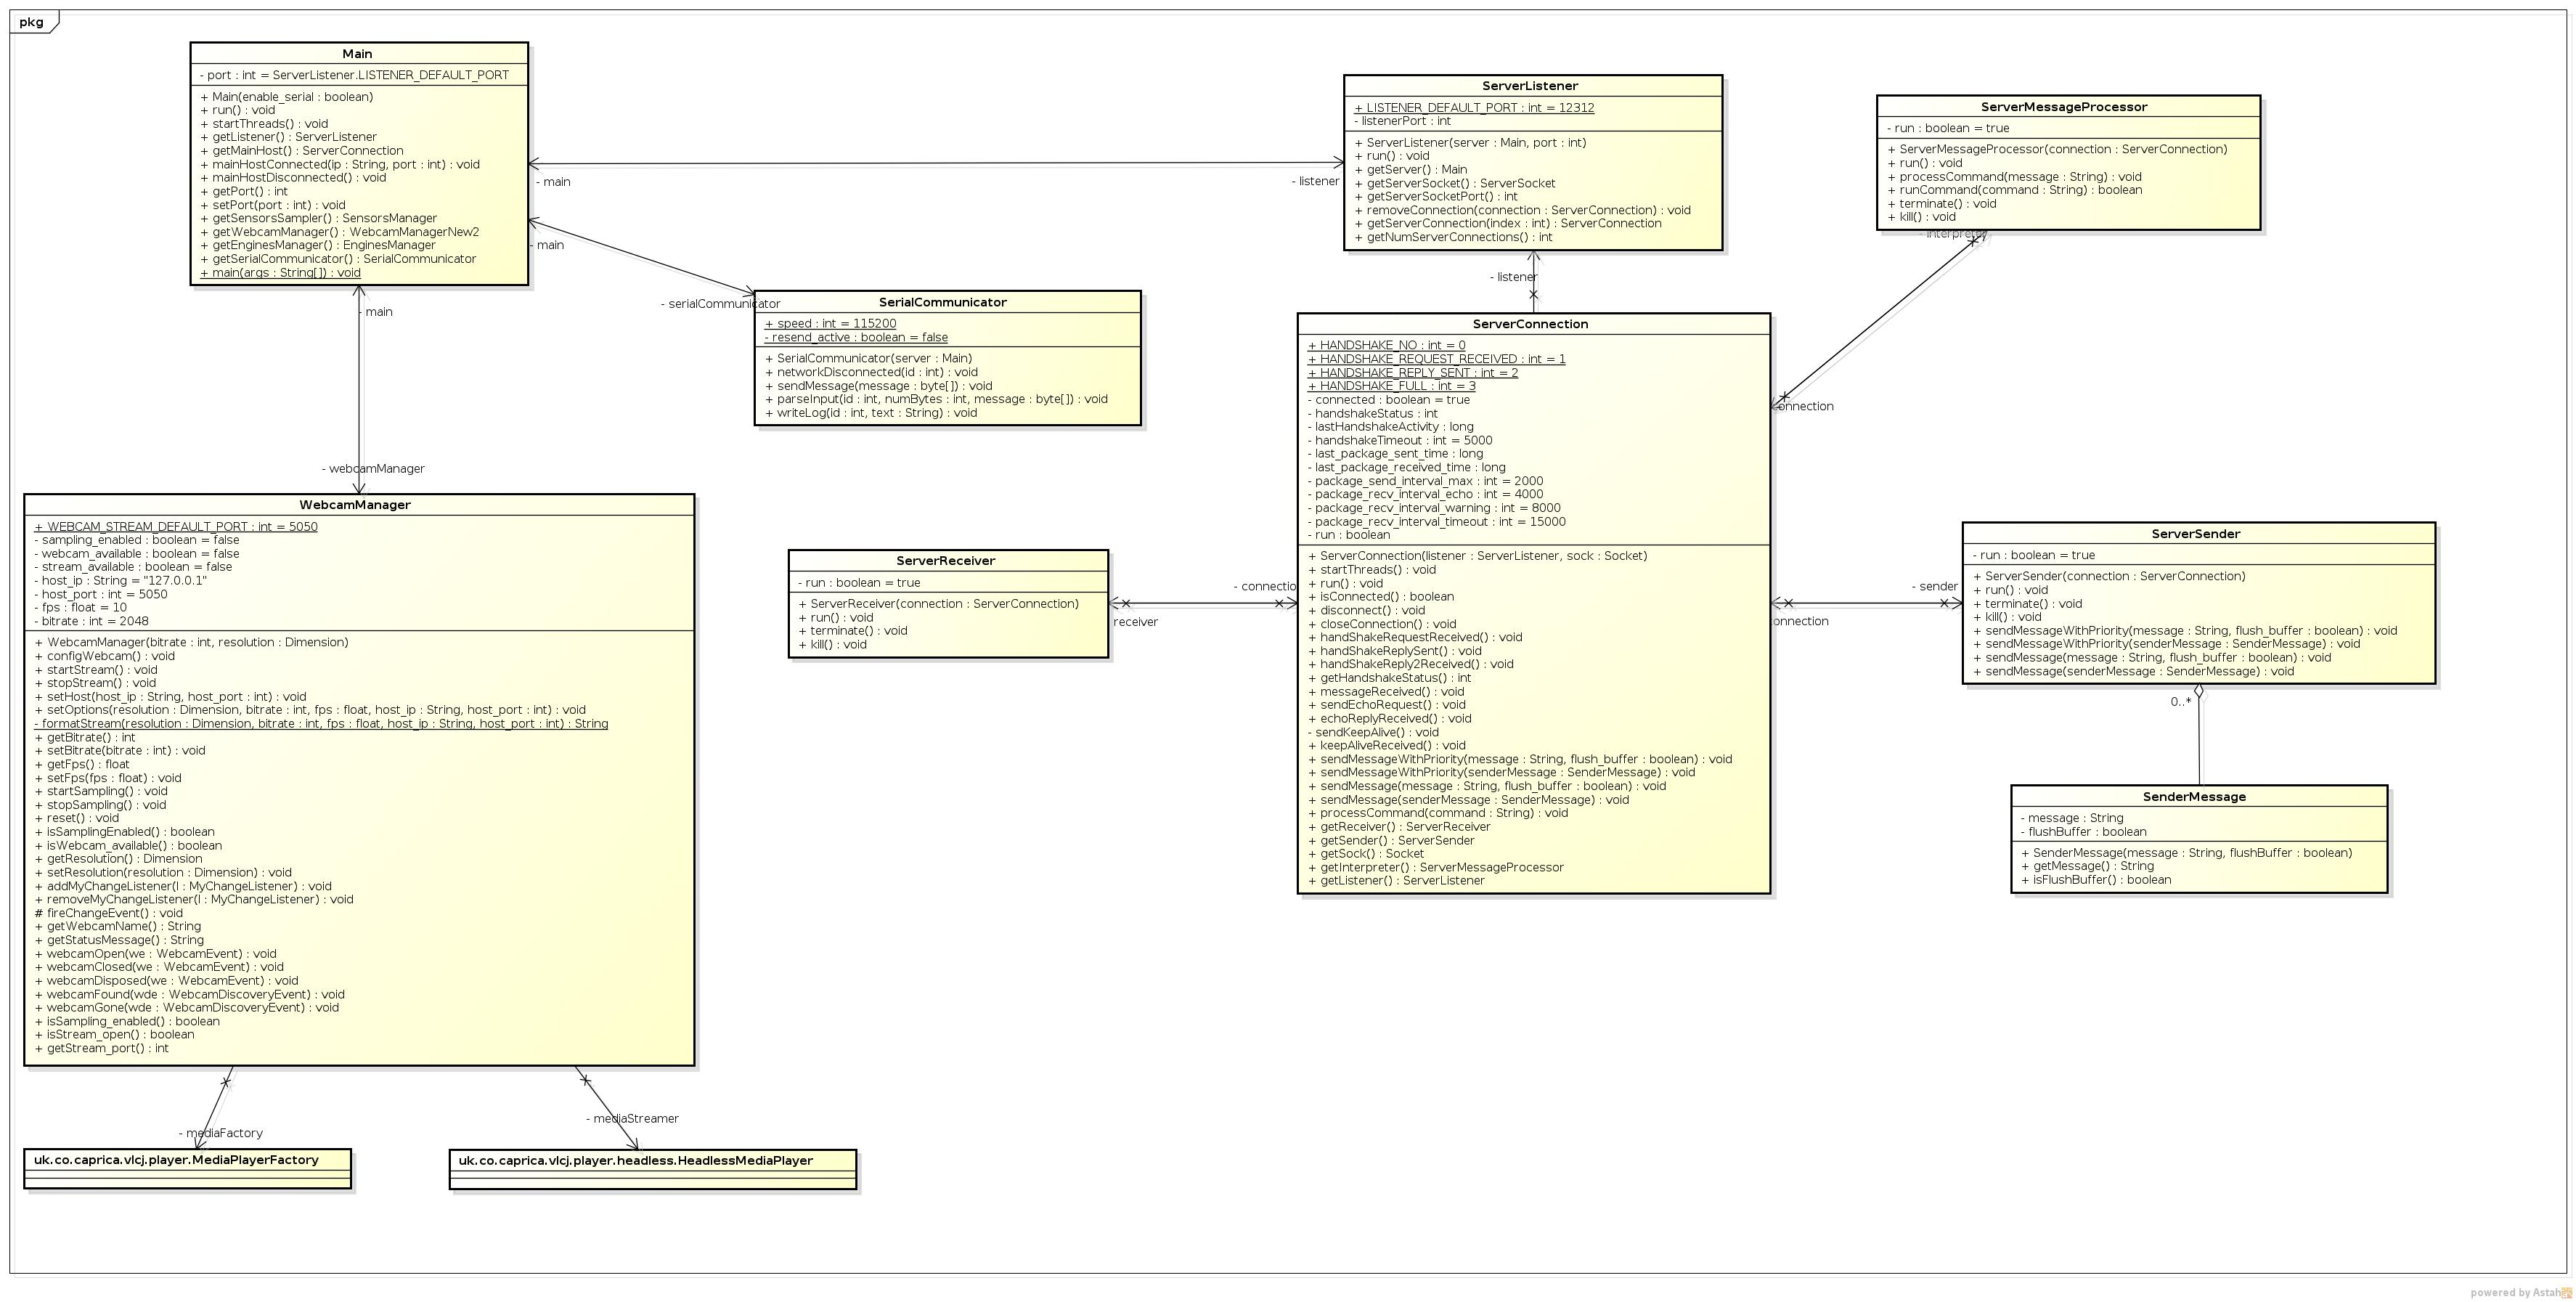
\includegraphics[width=\textwidth]{./figuras/sistEmbarcado/class_sistEmbarcado.jpg}
  \caption{Diagrama de classes do sistema embarcado (placa TS-7260).}
  \label{fig:diagrama_classes_sist_embarcado}
\end{figure}



%\subsection{Descrição das classes do sistema embarcado (TS-7260)}

\begin{table}[H]
  \centering
  \caption{Descrição das classes do sistema embarcado (placa TS-7260)}
  \begin{tabular}{p{6cm}p{8cm}}
    \toprule
    \textbf{Classe} & \textbf{Descrição} \\ 
    \midrule
   Main & Classe principal do robô. \\ \hline
   SensorsSampler & Thread responsável por requisitar amostras dos sensores da plca de baixo nível em intervalos de tempo previamente programados. \\ \hline
   ServerMessageProcessor & Thread responsável por realizar o processamento de mensagens recebidas de um host de conexão. \\ \hline
   ServerListener & Thread responsável por escutar requisições de conexão. \\ \hline
   ServerSender & Thread responsável por enviar mensagens ao host de uma conexão. \\ \hline
   SenderMessage & Contém uma mensagem que pode ser enviada por um Sender. \\ \hline
   ServerReceiver & Thread responsável por receber mensagens de um host de uma conexão. \\ \hline
   SerialCommunicator & Responsável por gerenciar a comunicação via porta serial entre a TS-7260 e a LPC2103.\\ \hline
   WebcamManager & Responsável por gerenciar a abertura e o fechamento da stream de imagens da webcam, além de configurar opções como resolução e taxa de frames. \\
   \bottomrule
  \end{tabular}%
  \label{tab:classes_ts}%
\end{table}%

\section{Cronograma original versus executado}
O cronograma original (Anexo D), foi executado conforme o esperado. Devido à antecipação de certas tarefas, eventuais atrasos ficaram dentro do planejado. Os deliverables foram entregues dentro do prazos estipulados.

\section{Orçamento original versus executado}
Como pode ser visto no orçamento em anexo, o custo total do projeto ficou em 899 reais, o que ultrapassou a inicial máxima em cerca de 18,9\%. Isso se deu, principalmente devido à ocorrência do risco de ``Taxação dos componentes comprados no exterior'', o que elevou signif
\chapter{Conclusões}

\section{Análise do desenvolvimento}

Do ponto de vista dos objetivos, percebe-se que a maioria deles foram alcançados. Foi implementado com sucesso um \textit{software} com interface gráfica para geração e visualização de mapas, visualização de imagens da \textit{webcam} do robô e controle do robô por meio do teclado. A comunicação foi implementada satisfatoriamente, tanto entre a estação base e a placa TS-7260 (via Wi-Fi) quanto entre a TS e a placa de baixo nível, via porta serial. Uma \textit{webcam} USB foi instalada e configurada com sucesso no robô para a transmissão de imagens ao usuário. O giroscópio foi utilizado satisfatoriamente na prática para corrigir erros de leituras dos encoders e escorregamento das rodas. Uma placa de circuito impresso, de tamanho reduzido, foi desenvolvida de forma a integrar as funções de baixo nível do robô: interface com os encoders, sensores infra-vermelhos, acelerômetro e giroscópio, e geração de PWM para os motores.

Observou-se que três riscos previstos no planejamento de riscos ocorreram. O primeiro foi a ``Não entrega de componentes ou entrega fora do prazo''. Uma unidade MPU-6050 (acelerômetro e giroscópio) encomendada no site eBay não foi entregue da maneira especificada e foi devolvida. Como a encomenda desse item havia sido adiantada, realizou-se uma nova encomenda no site Sparksfun, que chegou no prazo estabelecido não causando atraso no projeto. O segundo risco foi ``Taxação dos componentes comprados no exterior'', que gerou um aumento no preço dos componentes, mas não de forma que ultrapassasse o orçamento especificado. O terceiro e último risco foi ``Problemas Técnicos com o Hardware''. Como relatado, a imprecisão da leitura dos encoders ópticos interferiu na correta determinação da posição do robô. Como solução, buscou-se aumentar a aderência das rodas e correias do robô a fim de diminuir os escorregamentos e falsas leituras, além de utilizar o giroscópio para correção do posicionamento.

Em termos de déficts de conhecimento, pode-se citar a dificuldade em se utilizar o acelerômetro da placa, devido a seus problemas de leitura. Idealmente, o filtro de Kalman poderia ser utilizado para produzir melhores estimativas do posicionamento do robô, houve falta de tempo e base acadêmica para implementação desse filtro, que, na prática mostrou-se complexo de complexa interpretação e aplicação.

Por último, devido a um bom planejamento do cronograma, da execução da equipe e da baixa ocorrência de riscos, não houve atrasos dentro do cronograma planejado. As atividades foram concluídas dentro do prazo previsto pela equipe.

\section{Integração}

Para o desenvolvimento do projeto, da matéria de Oficinas de Integração 3, foram necessários diversos conhecimentos adquiridos durante o curso. Foram utilizados, principalmente, os conhecimentos nas áreas de Eletrônica Geral, Programação, Engenharia de Software e Comunicação de Dados.

O projeto foi dividido em três seções cada uma com sua gama de conhecimentos específicos:

Planejamento do Projeto: Nesta seção foram utilizados conhecimentos como Gerenciamento de Risco, Custo, Cronograma, Análise Tecnológica, entre outros, adquiridos nas matérias de Análise de Projeto de Sistemas, Engenharia de Software, Oficinas de Integração 1 e 2. Esses conhecimentos foram aplicados para criar o cronograma do projeto considerando a possibilidade de riscos e os custos e trabalho necessário para concluí-lo.

Hardware: Nesta seção foram utilizados conhecimentos como Microcontroladores, Sensores, Filtros, Sinais, Circuitos Digitais , entre outros, adquiridos nas matérias de Eletrônica, Microcontrolados, Controle, Sinais e Sistemas. Esses conhecimentos foram aplicados no desenvolvimento e na confecção da placa de circuito impresso, no uso e controle do robô, etc.

Software: Nesta seção foram utilizados conhecimentos como Programação, Comunicação de Dados, Estrutura de Dados. Esses conhecimentos foram aplicados para criar o programa da estação base, assim como possibilitar toda a estrutura de comunicação entre as partes do projeto.

\section{Trabalhos futuros}

Há inúmeros modos de se prosseguir com o projeto do robô Bellator, pois muitas melhorias podem ser efetuadas a fim de se atingir resultados mais precisos em termos de mapeamentos de ambientes.

No que diz respeito ao sensoriamento, é importante melhorar a confiabilidades dos dados dos encoders. Uma das formas de se fazer isso é utilizando um \textit{timing belt}, que é uma roda dentada acoplada a um sensor. Dessa forma, problemas de escorregamento da correia em relação à polias do robô seriam eliminados.

Quanto ao uso do acelerômetro, a técnica do filtro de Kalman poderia ser explorada se forma a se realizar a fusão de dados dos três sensores do robô: encoder, acelerômetro e giroscópio. Se desenvolvida corretamente, em tese, a utilização desta técnica permitiria a compensação automática de erros dos sensores o que permitiria uma estimativa muito melhor do posicionamento do robô. As dificuldades de se utilizar esta técnica são: correta determinação da margem de erro de cada sensor, criação de um modelo matemático da movimentação do robô e complexidade do entendimento e implementação do filtro.

Em relação à câmera, há dois aspectos a serem melhorados: a redução do atraso do sinal de vídeo (que é da ordem de segundos) e a interação do usuário com a câmera. O primeiro problema poderia ser resolvido com a substituição da \textit{webcam} atual por outra que possua menos latência, ou pelo desenvolvimentos de software que faça a leitura dos dados brutos da câmera e faça o envio instantâneo desses dados à estação base, procurando reduzir ou eliminar a utilização de \textit{buffers} de vídeo. Em termos de interatividade, pode-se construir um dispositivo de rotação que permita ao usuário girar a câmera 360 graus em torno do eixo vertical, possibilitando maior flexibilidade e autonomia durante a utilização do robô.
\apendice

%Neste capítulo estão expostos os riscos previstos para o projeto.

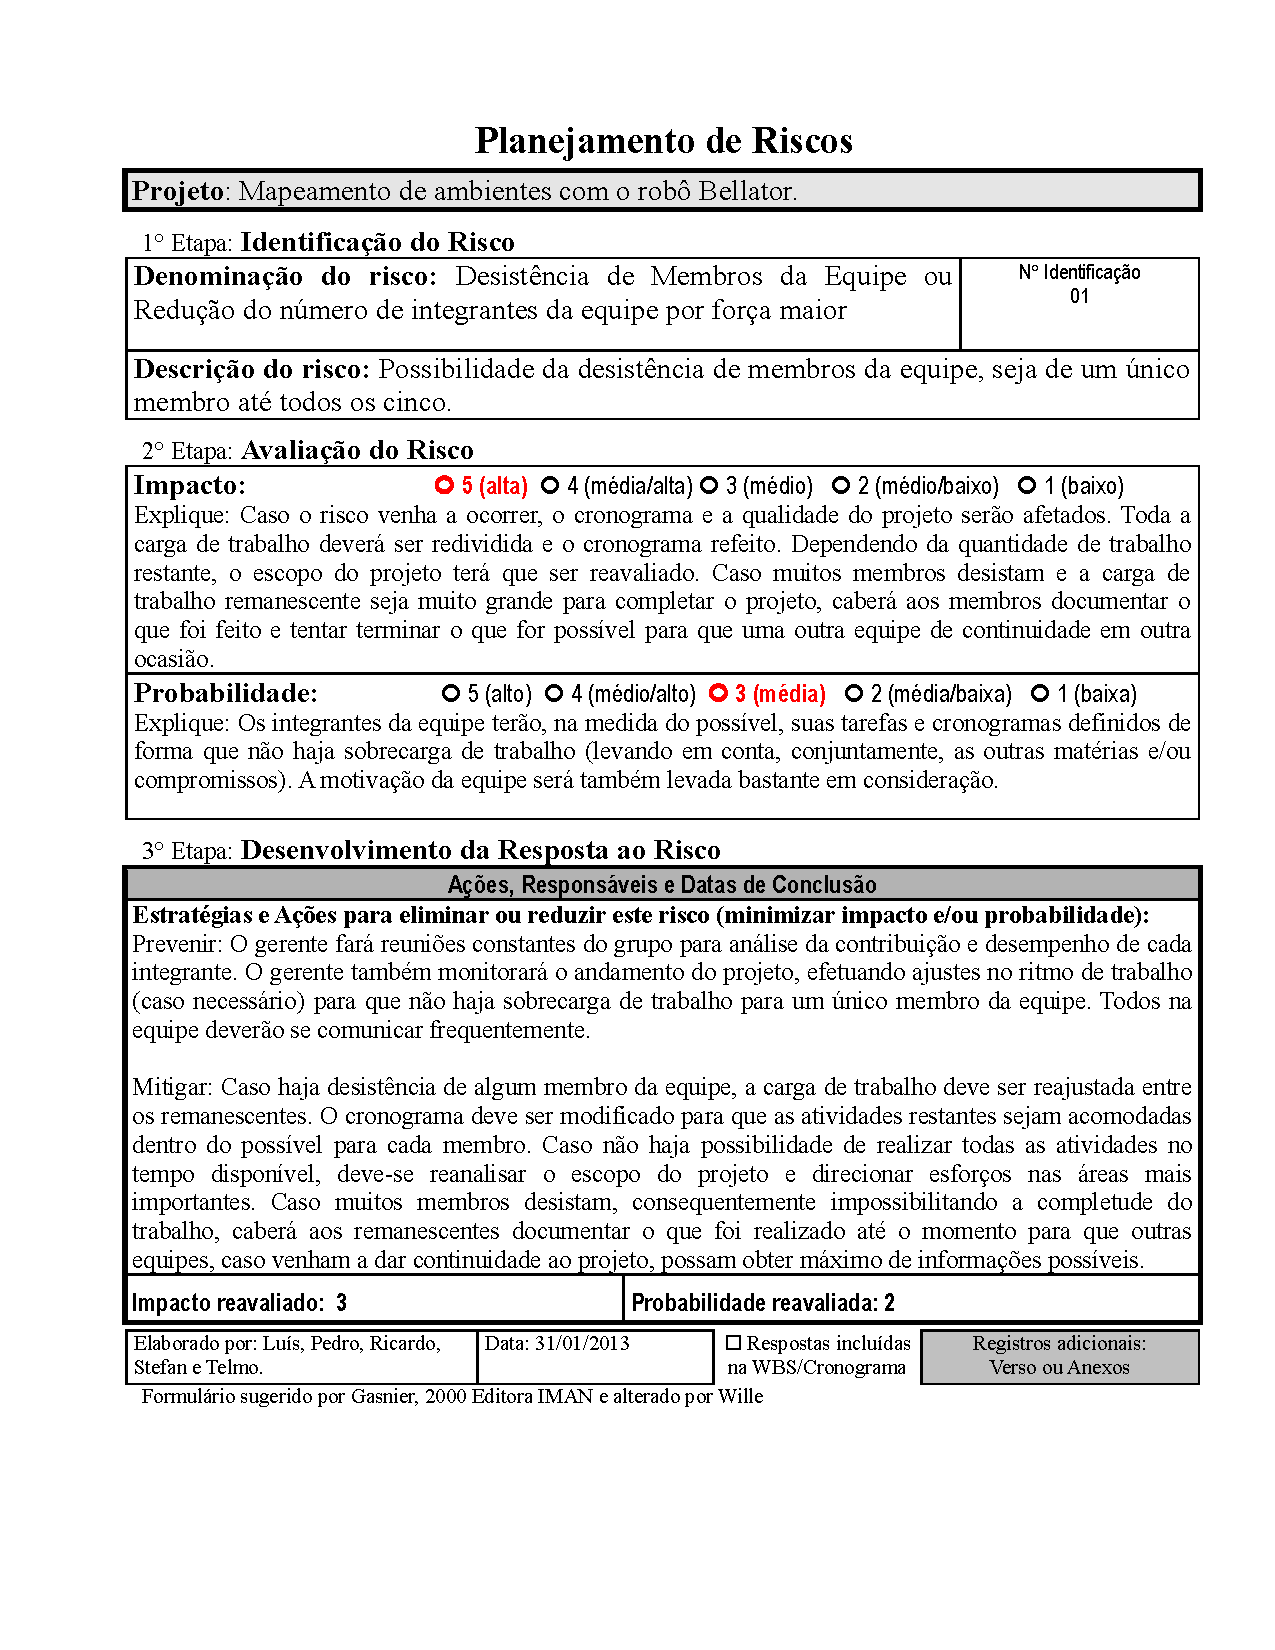
\includepdf[pages=1,scale=0.5, pagecommand=\chapter{Planejamento de riscos}]{Planejamento_de_Riscos_v3.pdf}
\includepdf[pages=2-9, pagecommand=]{Planejamento_de_Riscos_v3.pdf}


\chapter{Medidas do robô}
\label{cap:medidas_robo}
% Na Tabela \ref{tab:medidas_robo} estão presentes as medidas do robô.

\begin{table}[H]
  \caption{Medidas do robô.}
  \centering
  \begin{tabular}{l|l}
    \toprule
    \textbf{Medida} & \textbf{Valor} \\
    \midrule
    Comprimento da carcaça & 50 cm \\ \hline
    Largura da carcaça & 40 cm \\ \hline
    Distância entre a parte da frente do robô e os eixos das rodas & 14 cm \\ \hline
    Largura de cada roda & 4 cm \\ \hline
    Circunferência de cada roda & 64 cm \\ \hline
    Circunferência do eixo de cada roda & 7,5 cm \\ \hline
    Circunferência do eixo de cada encoder & 22 cm \\ 
    \bottomrule
  \end{tabular}
  \label{tab:medidas_robo}
\end{table}

\chapter{Diagramas detalhados de hardware}
\section{Diagrama elétrico/eletrônico}

Na figura \ref{fig:diagrama_eletrico_eletronico} mostra-se o diagrama de elétrico eletrônico do sistema embarcado. Cada bloco da figura \ref{fig:diagrama_blocos_hardware} corresponde a alguns componentes do diagrama elétrico eletrônico. A seguir detalha-se um pouco mais cada bloco.

\begin{figure}[H]
  \centering
  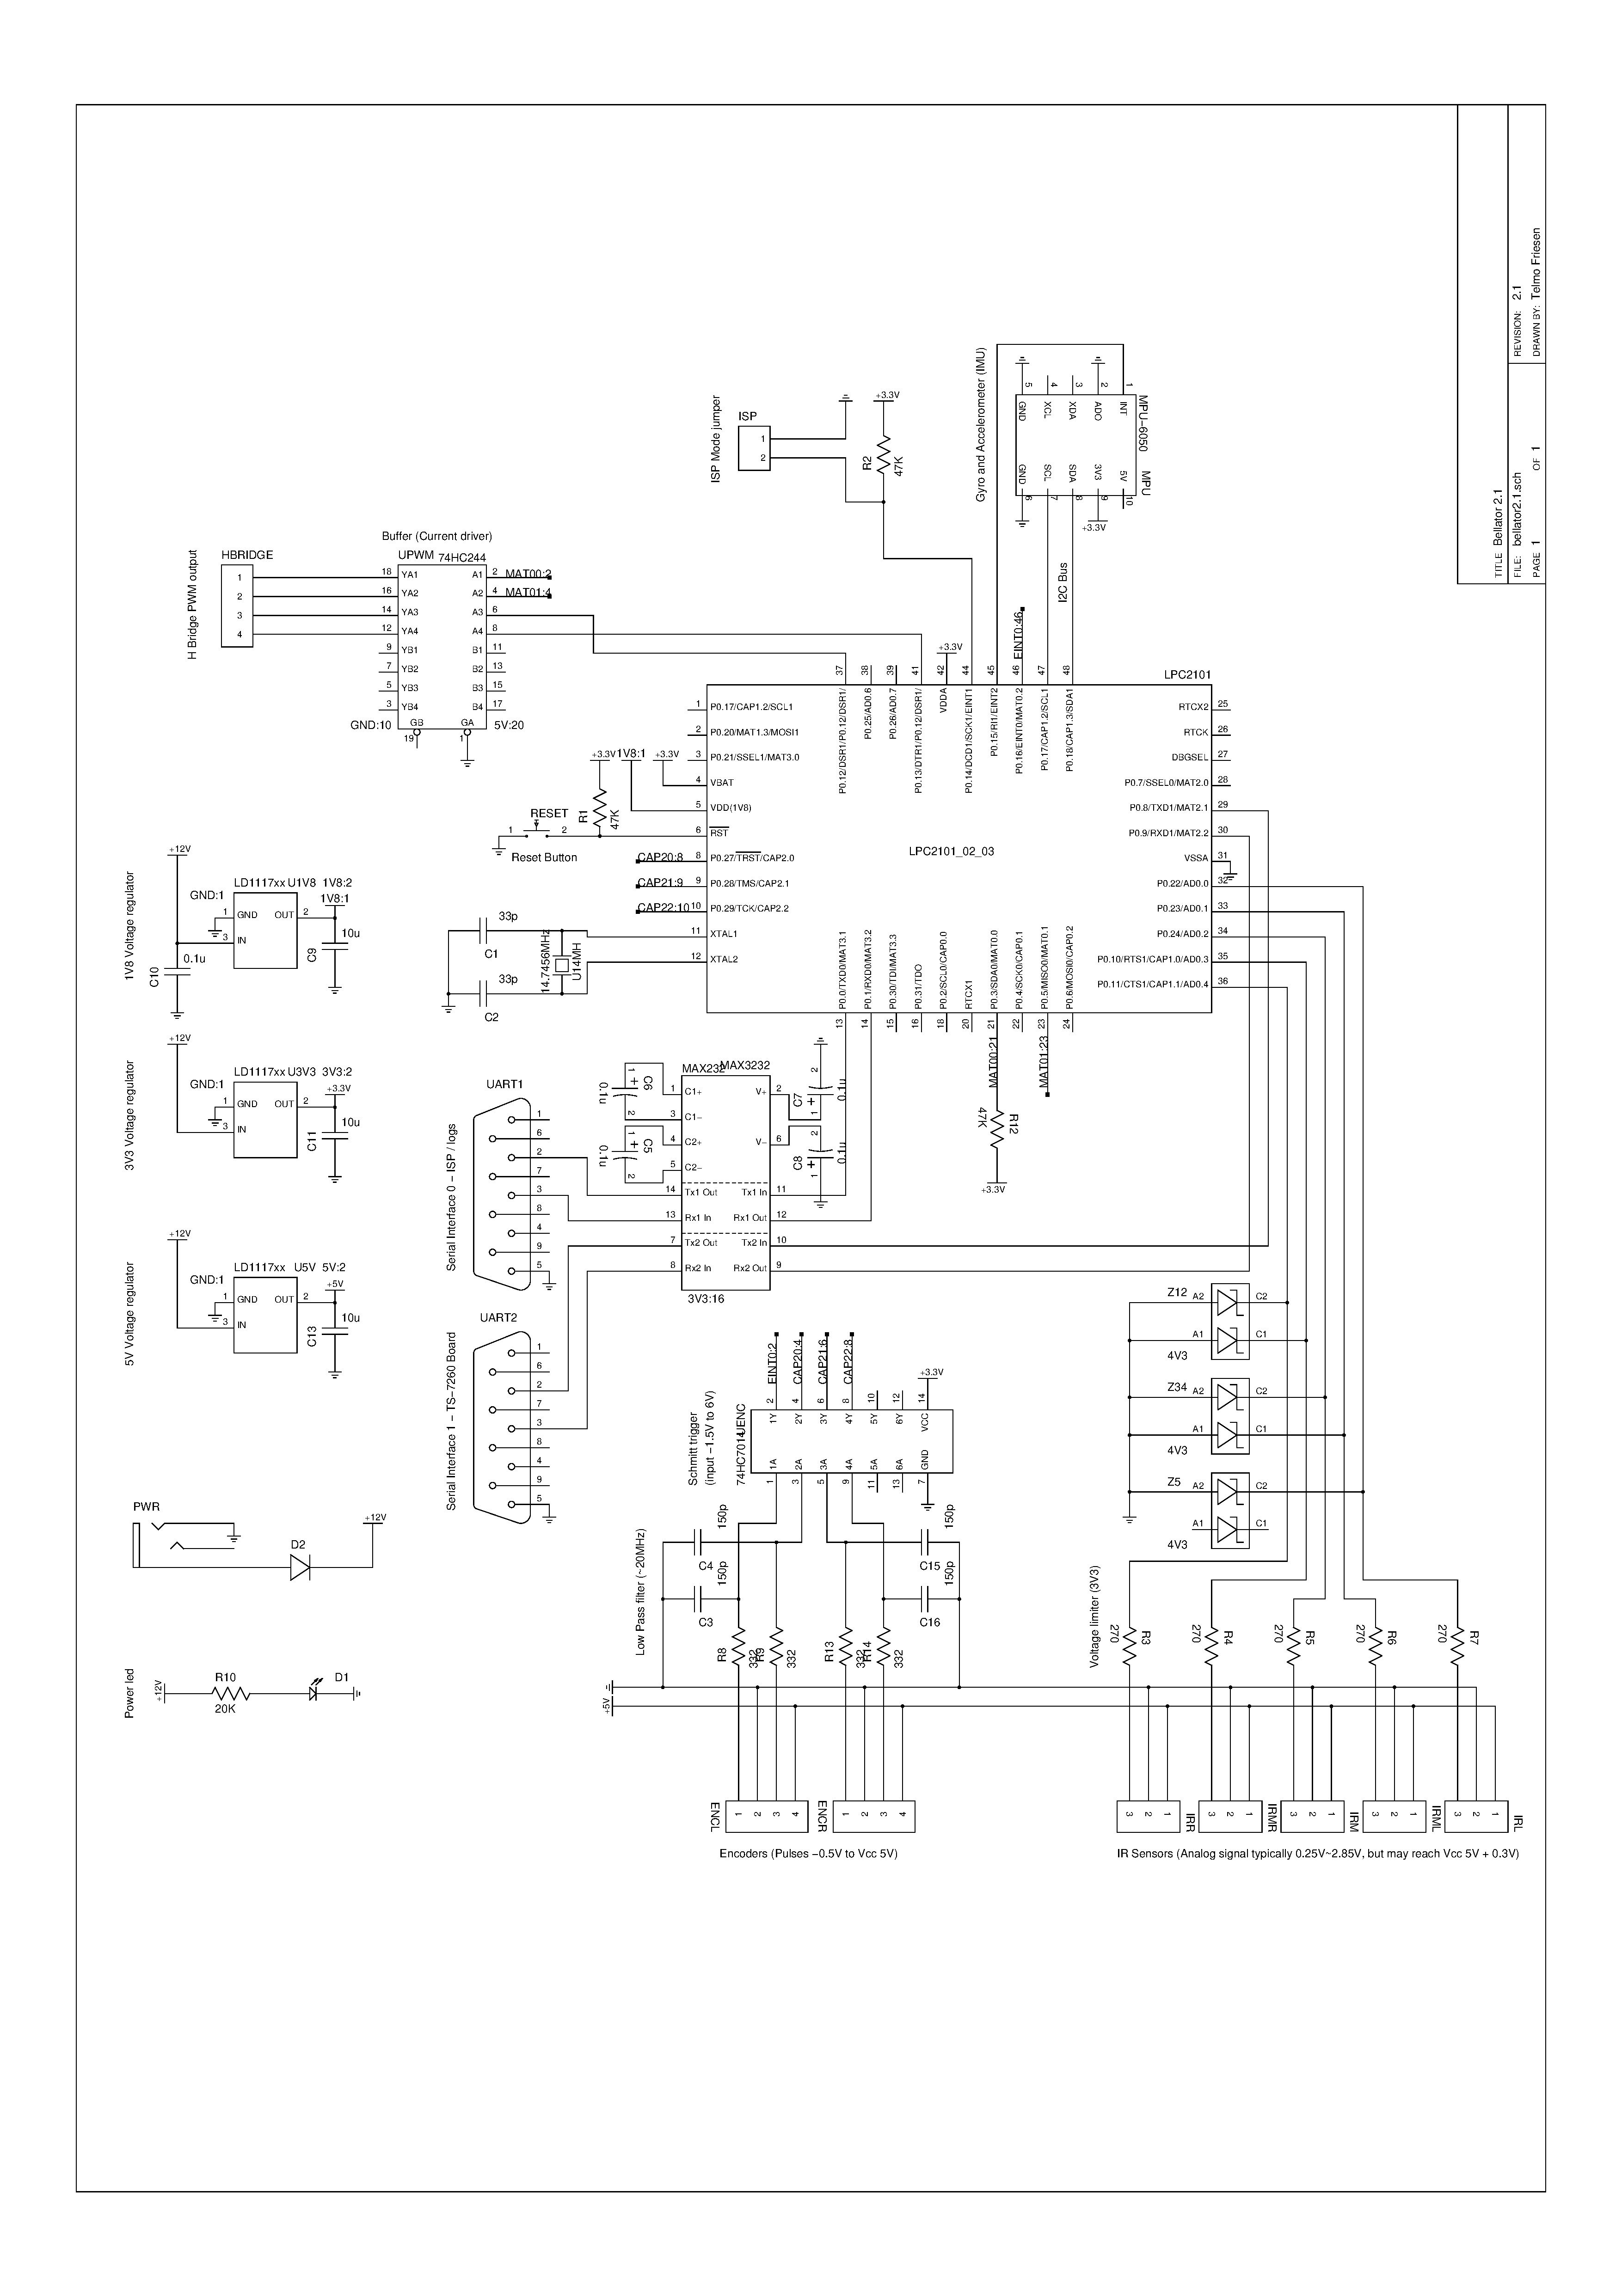
\includegraphics[width=0.9\textwidth, keepaspectratio]{./figuras/hardware/hardware2_2.pdf}
  \caption{Diagrama elétrico/eletrônico.}
  \label{fig:diagrama_eletrico_eletronico}
\end{figure}

\begin{enumerate}[topsep=0pt, partopsep=0pt, itemsep=0pt]
    \item Microcontrolador: Composto pelo microcontrolador LCP2103 da NXP que possui arquitetura ARM. Ele dispõe de duas interfaces seriais, conversor analógico digital com 8 canais, interface i2c, entradas de captura e interrupção, saídas de PWM entre outras funções que não serão utilizadas nesse projeto.
    \item UART 0/1: Constituído por um chip max3232 que opera em níveis de tensão CMOS e que gera os níveis adequados para o padrão RS-232 utilizando alguns capacitores.
    \item Buffer: Constituído por um chip 74HC244, é responsável por fornecer corrente e elevar os níveis de tensão de saída do microcontrolador de 3,3V para 5,0V.
    \item IMU: Composto pela placa de desenvolvimento MPU-6050, que possui um chip com o mesmo nome, MPU-6050, e circuitos RC auxiliares necessários para o funcionamento do MPU-6050.
    \item Limitador de tensão: Constituído de um resistor com baixo valor, 270 ohms, e um diodo Zener polarizado reversamente e com tensão de ruptura de 4.3V. Quando a tensão de entrada ultrapassar 4.3V o diodo passa a conduzir e mantém a tensão de 4.3V no resistor. O datasheet do microcontrolador sugere que se mantenha a impedância da carga menor que 40kohms, logo a adição de um resistor de 270 ohms pode ser desconsiderado com relação ao erro que possa causar na leitura do conversor. Um resistor de 270 ohms leva a uma corrente de 3.7mA quando a saída do sensor for 5.3V, que é o valor máximo previsto no datasheet.
    \item Tratamento de sinal: Composto por um filtro RC passa baixas e um chip 74HC7014. As frequências acima de 20MHz são atenuadas no sinal do encoder. Esse valor foi calculado com base na forma de onda da saída especificada no datasheet do encoder. Para tanto utilizam-se resistores de 332 ohms e capacitores de 150pF.
\end{enumerate}


\section{Placa de circuito impresso}

O projeto da placa de circuito impresso (PCB) do sistema embarcado de baixo nível está explicitado nas Figuras \ref{fig:pcb_cima} e \ref{fig:pcb_baixo}. Na Figura \ref{fig:pcb_pronta} está presente uma foto da placa pronta com os componentes soldados.

\begin{figure}[H]
  \centering
  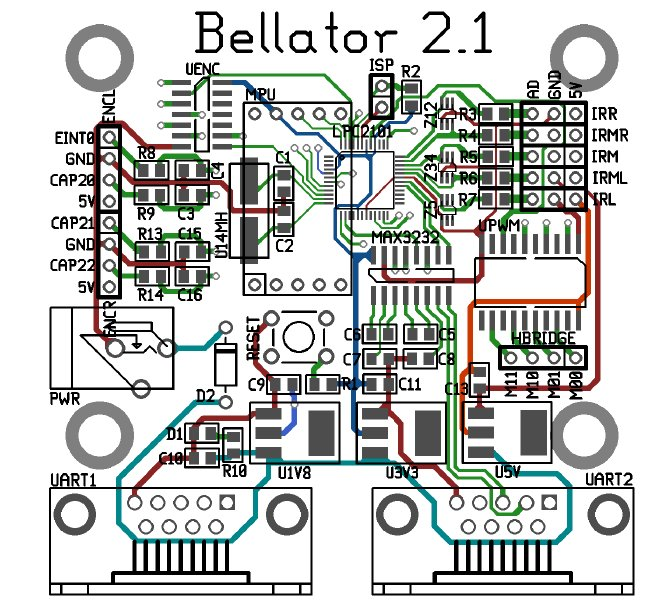
\includegraphics[width=0.7\textwidth, keepaspectratio]{./figuras/hardware/pcb_cima.jpg}
  \caption{Projeto da PCB -- lado de cima.}
  \label{fig:pcb_cima}
\end{figure}

\begin{figure}[H]
  \centering
  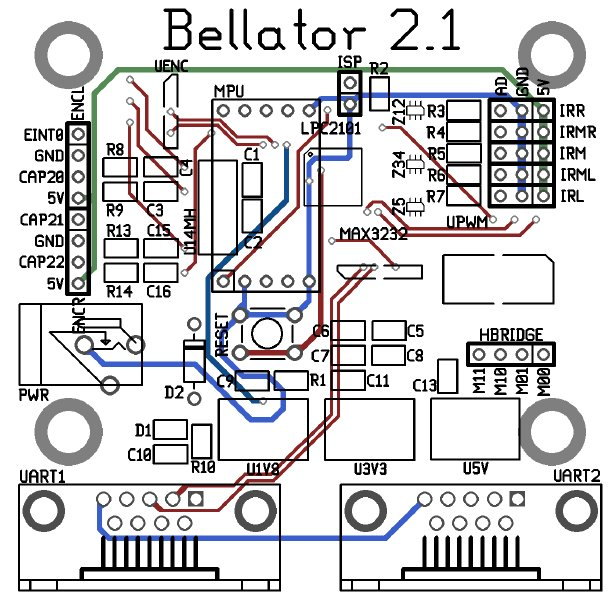
\includegraphics[width=0.7\textwidth, keepaspectratio]{./figuras/hardware/pcb_baixo.jpg}
  \caption{Projeto da PCB -- lado de baixo.}
  \label{fig:pcb_baixo}
\end{figure}

\begin{figure}[H]
  \centering
  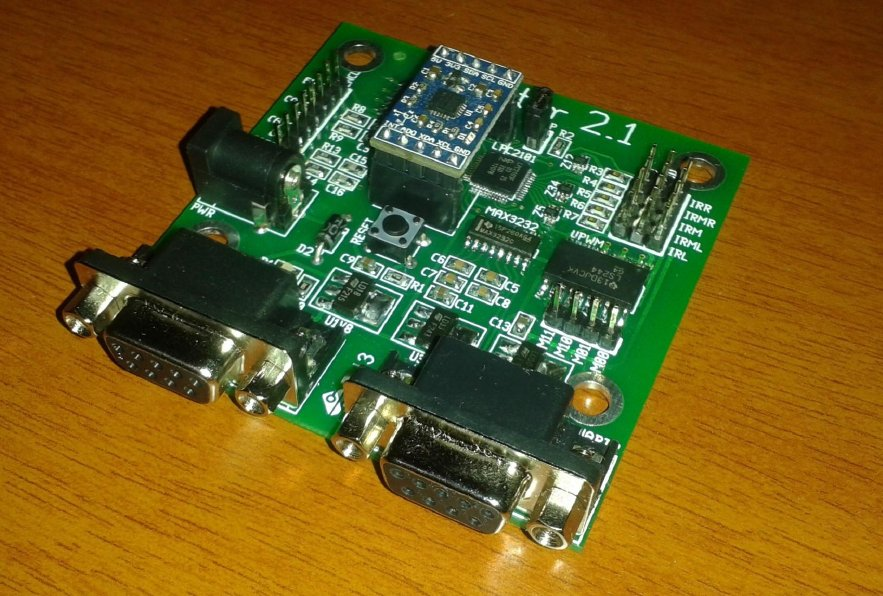
\includegraphics[width=0.7\textwidth, keepaspectratio]{./figuras/hardware/pcb_pronta.jpg}
  \caption{PCB montada.}
  \label{fig:pcb_pronta}
\end{figure}

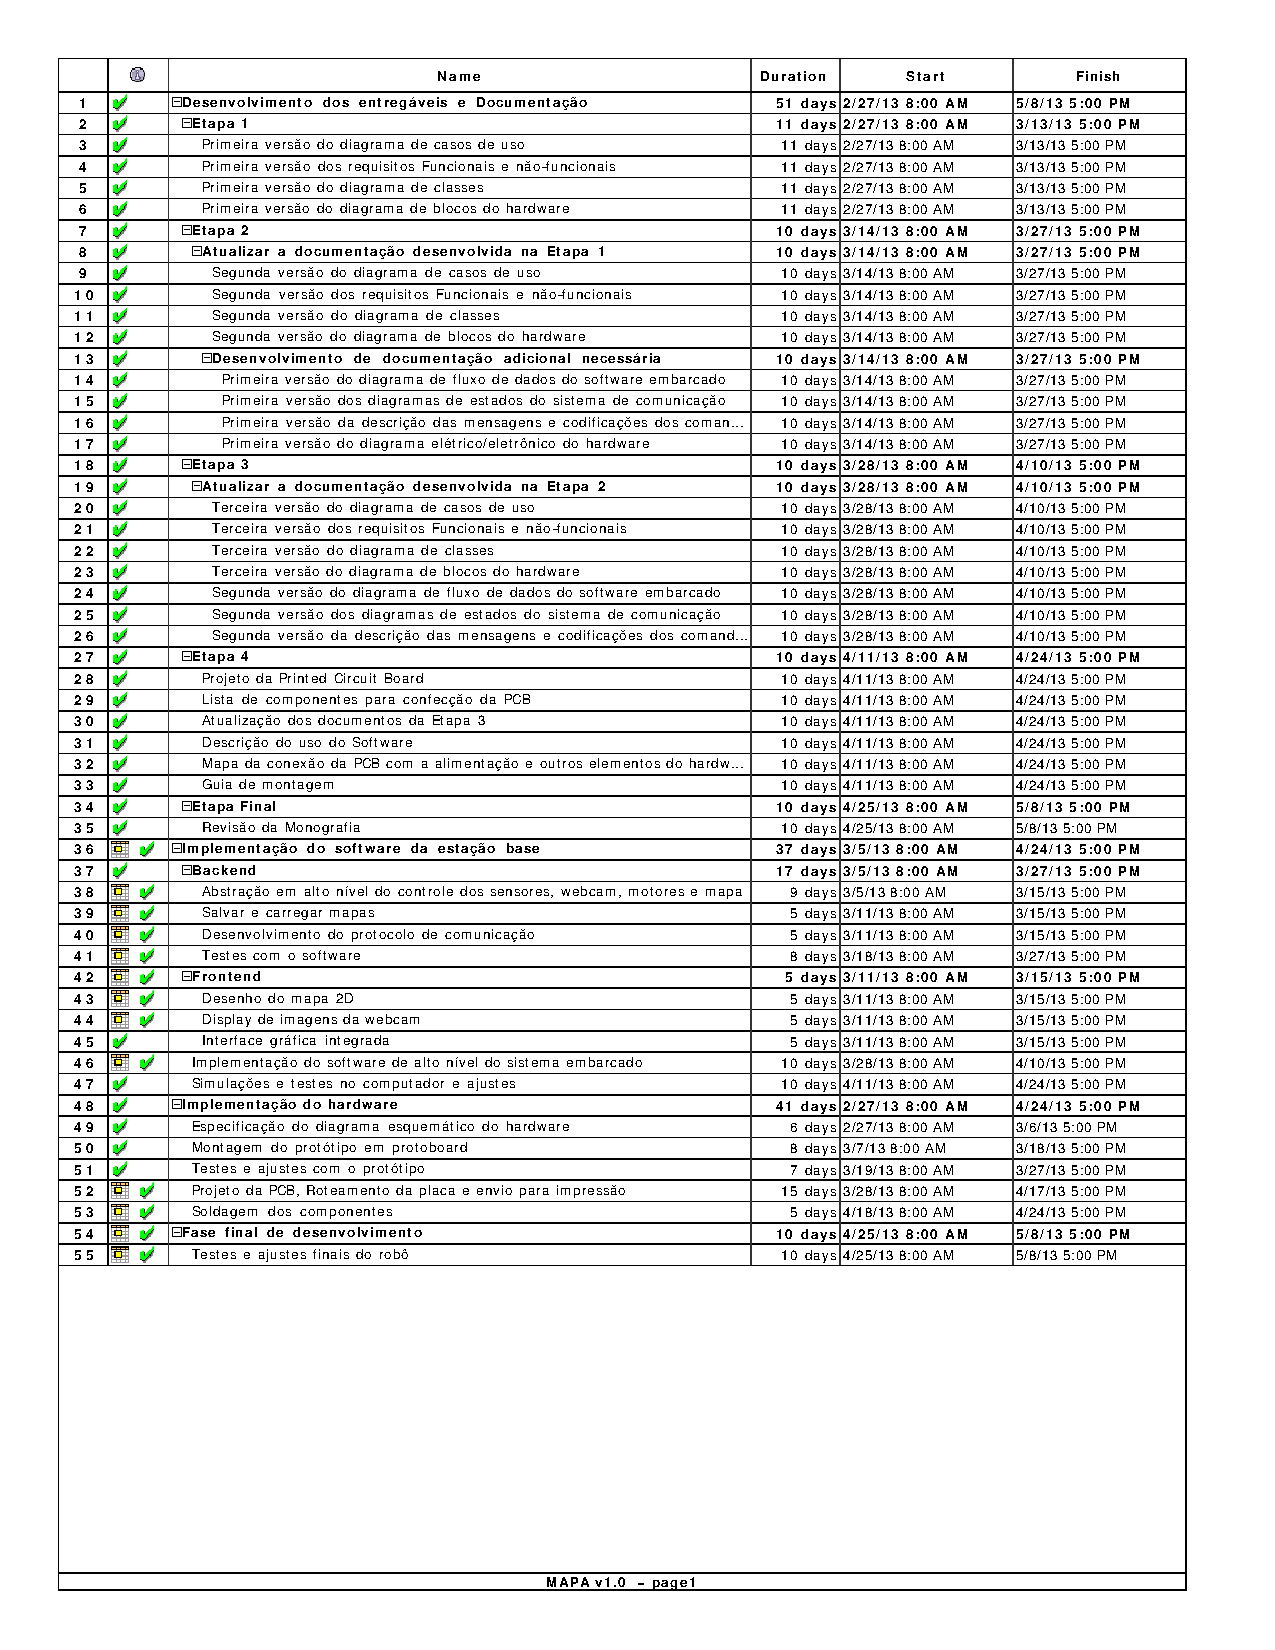
\includepdf[pages=1,offset=0 -130, pagecommand=\chapter{Cronograma}]{cronograma.pdf}

\raggedright

\bibliography{referencias}

\end{document}

